\documentclass[11pt]{article}

% ==== PAGE GEOMETRY (matches QF journal: 160mm x 230mm type area) ====
\usepackage[
  textwidth=160mm, textheight=230mm,
  top=32mm, headheight=5pt, headsep=19pt, footskip=32pt
]{geometry}

% ==== FONTS (Times Roman, matching QF style) ====
\usepackage[T1]{fontenc}
\usepackage{mathptmx}

% ==== MATH ====
\usepackage{amsmath,amssymb,amsthm}

% ==== BIBLIOGRAPHY ====
\usepackage[round,authoryear]{natbib}

% ==== TABLES & FIGURES ====
\usepackage{graphicx,booktabs,rotating,multirow,tabularx,placeins}
\usepackage{xcolor}

% ==== LISTS ====
\usepackage{enumerate}

% ==== SECTION HEADINGS (QF style: bold, 11/13pt) ====
\usepackage{titlesec}
\titleformat{\section}
  {\fontsize{11}{13}\selectfont\bfseries\raggedright}{\thesection.}{0.5em}{}
\titleformat{\subsection}
  {\fontsize{11}{13}\selectfont\bfseries\itshape\raggedright}{\thesubsection.}{0.5em}{}
\titlespacing*{\section}{0pt}{26pt plus 4pt minus 2pt}{13pt}
\titlespacing*{\subsection}{0pt}{24pt plus 3pt minus 2pt}{7pt}

% ==== TYPOGRAPHY ====
\setlength{\parindent}{10pt}
\setlength{\parskip}{0pt}
\setlength{\emergencystretch}{2em}

% ==== TITLE (18/22pt bold uppercase, centred, like QF) ====
\makeatletter
\renewcommand{\maketitle}{%
  \clearpage\null
  \vspace*{42pt}%
  \begin{center}
    {\fontsize{18}{22}\selectfont\bfseries\MakeUppercase{\@title}\par}%
    \ifx\@author\@empty\else
      \vskip 21pt
      {\fontsize{13}{15}\selectfont\@author\par}%
    \fi
  \end{center}
  \vskip 18pt
}
\makeatother

% ==== ABSTRACT (9/11pt, indented 2pc both sides) ====
\renewenvironment{abstract}{%
  \fontsize{9}{11}\selectfont
  \setlength{\leftskip}{2pc}%
  \setlength{\rightskip}{2pc}%
  \noindent\ignorespaces
}{%
  \par\addvspace{32pt}%
}

% ==== KEYWORDS (9/11pt, indented, italic label) ====
\newenvironment{keywords}{%
  \par\addvspace{11pt}%
  \fontsize{9}{11}\selectfont
  \setlength{\leftskip}{2pc}%
  \setlength{\rightskip}{2pc plus 1fill}%
  \noindent{\itshape Keywords\/}: \ignorespaces
}{%
  \par\addvspace{26pt plus 4pt}%
}

% ==== JEL CLASSIFICATION (same style as keywords) ====
\newenvironment{classcode}{%
  \par\addvspace{-9pt}%
  \fontsize{9}{11}\selectfont
  \setlength{\leftskip}{2pc}%
  \setlength{\rightskip}{2pc plus 1fill}%
  \noindent{\itshape JEL Classification\/}: \ignorespaces
}{%
  \par\addvspace{26pt plus 4pt}%
}

% ==== HYPERLINKS ====
\usepackage[colorlinks=true,linkcolor=blue,citecolor=blue,urlcolor=blue]{hyperref}

% ==== OPTIONAL RESULT-SCRIPT PROVENANCE ====
% Change the next line to \showresultscriptpathstrue to print the generating
% script below each numerical table or figure. Keep it false for submission.
\newif\ifshowresultscriptpaths
\showresultscriptpathsfalse
\newcommand{\resultscript}[1]{%
  \ifshowresultscriptpaths
    \par\smallskip
    {\raggedright\footnotesize\itshape Result-generation script: \path{#1}\par}%
  \fi
}

% ==== APPENDICES (renames sections to "Appendix A: ...") ====
\newcommand{\appendices}{%
  \appendix
  \titleformat{\section}
    {\fontsize{11}{13}\selectfont\bfseries\raggedright}
    {Appendix \thesection:}{0.5em}{}%
}

% ==== CUSTOM COMMANDS ====
\newcommand{\proofref}[1]{%
  \par\noindent\hfill{\small\itshape\hyperref[#1]{$\triangleright$ Proof, p.\,\pageref{#1}}}}
\newcommand{\E}{\mathbb{E}}
\renewcommand{\P}{\mathbb{P}}
\newcommand{\R}{\mathbb{R}}
\newcommand{\diff}{\mathrm{d}}
\newcommand{\F}{\mathcal{F}}
\newcommand{\one}{\mathbf{1}}
\newcommand{\Rea}{\operatorname{Re}}

% ==== THEOREM ENVIRONMENTS ====
\theoremstyle{plain}
\newtheorem{theorem}{Theorem}[section]
\newtheorem{lemma}[theorem]{Lemma}
\newtheorem{proposition}[theorem]{Proposition}

\theoremstyle{definition}
\newtheorem{definition}{Definition}[section]
\newtheorem{assumption}{Assumption}[section]

\theoremstyle{remark}
\newtheorem{remark}{Remark}

\begin{document}

\title{Evaluating Leveraged DeFi Long--Short Positions under Jump Risk: Killed Moments, Liquidation Recovery and the Limits of Optimal Sizing}

% TODO: author list (Francis Liu and co-author) before circulation.

\maketitle

\begin{abstract}
We develop a semi-analytic method for evaluating leveraged long--short positions held on DeFi
lending protocols, whose solvency is governed by a collateral-to-liability health factor and which
are liquidated when that factor falls below one. Under bivariate Kou jump--diffusion dynamics, an
exponential change of measure absorbs the short-leg price and reduces every admissible killed
payoff moment to a one-dimensional killed expectation of the log price ratio. Its Laplace-domain
resolvent is a $3\times3$ linear system for every moment order, and the survival probability is its
zero-order case. Bivariate tilts of the same system give the exact liquidation recovery under jump
overshoot, the law of the overshoot and with it the probability of bad debt, and the expected
logarithm of terminal wealth. The resulting \emph{evaluation map} from initial health buffer to
liquidation probability, payoff moments and recovery is validated against bridge-corrected Monte
Carlo and is two to three orders of magnitude faster. Applied to sizing on Aave v3, the map shows
that the optimal leverage is governed by a closed-form break-even drift of a few percent per year,
which the data cannot estimate precisely enough to act on. A model-free replay of $37$ Aave v3 pairs
over 2023--2026 under the protocol's liquidation rules points the same way: modest leverage beat
the unlevered position in $4$ pairs, never significantly. The replay also identifies the model's main
restriction: with independent jumps the calibration understates the legs' covariance, overstates
spread variance and biases the break-even.
\end{abstract}

\begin{keywords}
DeFi lending; leveraged long--short; health factor; killed payoff moments; Kou double-exponential jump diffusion; first-passage problem; Laplace resolvent; jump overshoot; bad debt; Kelly criterion
\end{keywords}

\begin{classcode}
G11; G12; C65
\end{classcode}

% ============================================================
\section{Introduction}
% ============================================================

Crypto-asset lending protocols such as Aave and Compound enable a leveraged long--short strategy: an
investor deposits one crypto asset as collateral, borrows a second, and sells it short. The position
is governed by a real-time \emph{health factor} --- a borrowing-power-adjusted ratio of collateral to
liability --- and is liquidated when that ratio falls below one. The exposure combines leveraged
relative-value risk, a path-dependent liquidation boundary, discontinuous price jumps and
state-dependent survival. Its initial health buffer controls both leverage and the distance to
liquidation, and evaluating that trade-off requires the distribution of a payoff killed at the
liquidation boundary, at every candidate buffer.

Two objects recur: the probability that the position survives to the horizon, and the moments of its
killed terminal payoff. Monte Carlo can approximate them, but barrier discretisation and sampling
noise are most consequential near liquidation, and repeated simulation is costly inside a sizing
search. What is missing is a fast, repeatable \emph{evaluation map} from the initial buffer to
survival probabilities, payoff moments and, once liquidation is priced, recovery --- an object that
any sizing rule needs and that is independent of the rule.

We construct this map under the Kou double-exponential jump--diffusion \citep{Kou2002}. Two
reductions make it semi-analytic. First, a unit-equity normalisation collapses the two holdings to a
single initial log health factor $h_0$, and liquidation depends only on the log price ratio
$Z=X_1-X_2$. Second, an exponential change of measure absorbs the short-leg price factor, so every
admissible payoff moment becomes a one-dimensional killed expectation of $Z$; because exponentials
are eigenfunctions of the Kou generator, its Laplace transform solves a $3\times3$ linear system
whose size does not grow with the moment order, and Talbot inversion \citep{Talbot1979} returns the
time-domain values.

The paper sits between the DeFi liquidation literature and the first-passage literature for jump
diffusions. \citet{Qin2021} and \citet{HeimbachHuang2024} document the incentive structure and
leverage amplification of DeFi liquidations empirically, without addressing ex-ante sizing.
\citet{KouWang2003} derive Laplace-transform first-passage results under double-exponential jumps,
and \citet{Sepp2004} reduces barrier option pricing to a finite algebraic system by the mechanism
used here; the finiteness is generic for exponential-type L\'evy models \citep{Cai2009,CaiKou2011,
AsmussenAvramPistorius2004}. We price a barrier-killed long--short \emph{ratio}, which the
change-of-numeraire tilt brings within reach of that machinery, and use bivariate tilts of the same
barrier system to obtain the joint law of the leg values at liquidation. More distantly,
\citet{JacobsLevyStarer1999} advocate joint optimisation of long and short legs and
\citet{DangForsyth2016} study dynamic mean--variance control under jump risk; our sizing problem is
a static analogue, optimising a single initial buffer against a killed-payoff distribution.

The paper makes five contributions.
\emph{(i)} It reduces the position to the scalar $h_0$ and constructs the objective-independent
evaluation map: the liquidation probability and every admissible killed moment $\E[\Pi_T^k]$ from
one $3\times3$ barrier system (Sections~\ref{sec:setup}--\ref{sec:resolvent},
Appendix~\ref{app:downward-phases}).
\emph{(ii)} It computes the exact liquidation recovery under jump overshoot from joint hitting
moments under bivariate tilts, and shows that the overshoot is a creeping atom plus two exponential
phases whose weights follow from three hitting moments; this gives the probability of bad debt in
closed form (Section~\ref{sec:recovery}).
\emph{(iii)} It evaluates the expected log of terminal wealth semi-analytically, so that Kelly
sizing needs no simulation (Section~\ref{sec:log-wealth}).
\emph{(iv)} It validates the map against an accuracy-matched, Brownian-bridge-corrected simulator
and, out of sample, against realised liquidation frequencies (Section~\ref{sec:numerical},
Appendix~\ref{sec:full-history}).
\emph{(v)} It applies the map to sizing. Under any of the usual objectives the optimal leverage is
decided by a closed-form \emph{break-even drift}; the data cannot estimate the drift well enough to
say whether it is exceeded; and a model-free replay of $37$ Aave v3 pairs shows that leverage rarely
paid ex post and that the model's independent-jump restriction biases its break-evens
(Section~\ref{sec:sizing}).
Interest-rate carry enters as a drift shift and, with a Markov-modulated rate regime, through a
$6\times6$ resolvent; both are small at a monthly horizon and are treated in
Appendix~\ref{app:carry}.

The framework abstracts from liquidation execution, dynamic collateral management and oracle
delays, and from protocol features that rescale the effective collateral factor or cap position
size (E-mode, supply/borrow caps, isolation mode). Section~\ref{sec:setup} defines the position and
the evaluation map; Section~\ref{sec:model} specifies the dynamics and tilt;
Sections~\ref{sec:moments}--\ref{sec:resolvent} derive the moments and their resolvent;
Section~\ref{sec:numerical} reports numerical results; Section~\ref{sec:recovery} adds recovery,
the overshoot law and expected log wealth; Section~\ref{sec:sizing} applies the map to sizing;
Section~\ref{sec:conclusion} concludes. The appendices give the downward-phase boundary conditions,
the calibration and its full-history validation, carry and regime switching, and the proofs.

% ============================================================
\section{Leveraged Long--Short Position and Health-Factor Barrier}\label{sec:setup}
% ============================================================

We consider a leveraged long--short portfolio in which an investor holds asset $S_1$
and owes asset $S_2$, with net initial equity normalized to one unit of account. The
position is liquidated if collateral becomes too small relative to the liability. This
section defines the barrier, the killed-payoff object studied in the paper, and the mapping
from the initial health buffer to holdings. No investor objective is needed for these
definitions.

\subsection{Health factor, liquidation time, and killed payoff}
Let $(\Omega,\F,(\F_t)_{t\ge 0},\P)$ be a filtered probability space.
Two strictly positive asset prices $S_1,S_2$ evolve as
\[
S_{i,t}=S_{i,0}e^{X_{i,t}},\qquad X_{i,0}=0,\quad i=1,2,
\]
where $X_1,X_2$ are log-price processes to be specified in Section~\ref{sec:model}.
The investor holds $n_1>0$ units of asset $S_1$ (long leg) and $n_2>0$ units of asset $S_2$ (short leg).

Let
\[
V_{1,t}:=n_1 S_{1,t},\qquad V_{2,t}:=n_2 S_{2,t}
\]
denote the \emph{collateral value} (long leg) and the \emph{borrow value} (outstanding liability) at
time $t$. Fix $b\in(0,1)$, the \emph{liquidation threshold} of asset $S_1$ (the Aave v3 parameter of the
same name; distinct from the maximum LTV at origination, which is a separate and typically lower
protocol constant). Solvency requires $V_{2,t}\le bV_{1,t}$; liquidation occurs when the
borrow value exceeds adjusted collateral,
\[
V_{2,t}>b\,V_{1,t}.
\]
The \emph{health factor} summarises this margin condition as a single ratio,
\begin{equation}\label{eq:health-factor}
H_t := \frac{b\,V_{1,t}}{V_{2,t}} = \frac{b\,n_1 S_{1,t}}{n_2 S_{2,t}},
\qquad
h_t := \log H_t,
\end{equation}
where $h_t$ is the \emph{log health factor}. The solvency condition is $H_t\ge 1$
($h_t\ge 0$); breaching it is equivalent to the borrow value exceeding the $b$-adjusted collateral.
Liquidation is triggered at the first such instant:
\[
\tau:=\inf\{t\ge 0:\;H_t<1\} = \inf\{t\ge 0:\;h_t<0\}.
\]
A larger $b$ permits a larger borrow-to-collateral ratio $V_2/V_1\le b$ before liquidation,
giving the position more room to absorb adverse price moves; a smaller $b$ is a stricter
protocol threshold, triggering earlier forced exit and limiting bad-debt exposure.

Since
\[
h_t
=
\log\!\Big(\frac{b\,n_1S_{1,0}}{n_2S_{2,0}}\Big)+(X_{1,t}-X_{2,t}),
\]
define the initial log health factor and the log-ratio process by
\[
h_0:=\log\!\Big(\frac{b\,n_1S_{1,0}}{n_2S_{2,0}}\Big),
\qquad
Z_t:=X_{1,t}-X_{2,t},
\]
so that $h_t=h_0+Z_t$ and the liquidation time is equivalently
\[
\tau=\inf\{t\ge 0:\; Z_t<-h_0\}.
\]
The one-dimensional process $Z$ thus carries all barrier-relevant risk: the position survives if and only if
$Z$ stays above the absorbing level $-h_0$. The parameter $h_0 = \log H_0$ is therefore the
\emph{initial log-cushion} — the log-distance of the initial health factor from the liquidation
boundary $H=1$. A larger $h_0$ means the position starts further from forced exit; $h_0\to 0^+$
means the position starts almost at the boundary with negligible cushion.

The \emph{killed terminal payoff} at horizon $T$ is
\[
\Pi_T:=(n_1S_{1,T}-n_2S_{2,T})\,\one_{\{\tau>T\}}.
\]
On $\{\tau>T\}$ the health factor satisfies $H_T\ge 1$, so $b\,n_1S_{1,T}\ge n_2S_{2,T}$;
since $b\in(0,1)$ this forces $n_1S_{1,T}>n_2S_{2,T}$, meaning the position carries strictly
positive terminal equity on every surviving path. No positive-part truncation is needed.
The indicator $\one_{\{\tau>T\}}$ assigns zero to liquidated paths. This defines a
\emph{killed payoff}; it is a mathematical convention rather than a model of the investor's
protocol-specific recovery.
Since the initial net book value is normalised to one unit of account (Section~\ref{sec:1d}),
net profit on a surviving path is $R_T:=\Pi_T-1$, but all moments in this paper are stated in
terms of $\Pi_T$ directly.
This paper characterises the killed moments of $\Pi_T$, the conditional distribution on
$\{\tau>T\}$, and the probability of that event, with $H_t=1$ treated as an absorbing
boundary. Section~\ref{sec:recovery} adds the recovery value of liquidated paths.

\begin{remark}[Liquidation convention]\label{rem:liquidation}
On Aave v3 a keeper may repay up to $50\%$ of the debt ($100\%$ below a secondary threshold) and
claims a liquidation bonus of $5$--$15\%$ of seized collateral; Compound is similar
\citep{Qin2021,HeimbachHuang2024}. Partial repayment, keeper timing, market liquidity and execution
prices all affect the value retained by the borrower. We treat the barrier as absorbing and set
$\Pi_T:=0$ on $\{\tau\le T\}$ to define the killed-payoff benchmark; a partial liquidation typically
restores $H>1$ and the position continues at reduced size, so absorption models a borrower who is
fully closed out. The zero is a bookkeeping convention, not a claim that recovery is worthless:
investor wealth is
\begin{equation}\label{eq:wealth}
W_T=\Pi_T+R_\tau\one_{\{\tau\le T\}},
\end{equation}
and Section~\ref{sec:recovery} computes the recovery $R_\tau$ exactly, including jump overshoot.
\end{remark}

\begin{remark}[Dynamic collateral management]\label{rem:dynamic}
A practitioner who monitors the health factor could top up collateral or partially unwind
the short leg to steer $H_t$ away from the liquidation boundary.
Such a strategy would replace the absorbing barrier with a reflecting or controlled
boundary and the static evaluation problem with a stochastic control problem. We hold the
position fixed to isolate the ex-ante killed-moment calculation; the assumption should not
be interpreted as a claim that dynamic intervention is infeasible or suboptimal. During a flash
crash --- the jump-driven event that dominates liquidation --- a position may be liquidated within
one or two blocks, before a remedial transaction confirms, so the static model is accurate for
stress episodes short relative to a monitoring cycle.
\end{remark}

\begin{remark}[Oracle prices]\label{rem:oracle}
Aave liquidates against Chainlink prices that update on a heartbeat or deviation threshold. Discrete
monitoring means a dip that recovers between updates does not liquidate, so the continuous barrier
\emph{overstates} liquidation frequency; but a stale oracle that gaps down liquidates at the gapped
level, so the continuous model \emph{understates} the recovery loss. Calibration prices are
reserve-level oracle-implied values (TVL divided by supplied balance).
\end{remark}

Thus killed payoff and investor terminal wealth are distinct objects. The former is the
tractable object evaluated below; recovery and intervention overlays may change the latter
and, consequently, any sizing decision built from it.

Using the definition of $H_T$, one obtains the following factorization.

\begin{lemma}[Payoff factorization]\label{lem:payoff-factor}
\begin{equation}\label{eq:payoff-factor}
\Pi_T
=
\frac{n_2}{b}\,S_{2,0}e^{X_{2,T}}\,(e^{h_0+Z_T}-b)\,\one_{\{\tau>T\}}.
\end{equation}
The factor $(e^{h_0+Z_T}-b)$ is strictly positive on $\{\tau>T\}$ because $H_T=e^{h_0+Z_T}\ge 1>b$,
consistent with the definition of $\Pi_T$.
\end{lemma}
This separates the payoff into a numeraire factor driven by $S_2$, and a barrier-killed option on the
log-ratio $Z$ with moneyness controlled by $h_0$.

\subsection{Health-buffer parameterization and feasible set}\label{sec:1d}

The two coin holdings $(n_1,n_2)$ represent two degrees of freedom. A normalization reduces
this to a single scalar, and the barrier structure identifies $h_0$ as the natural evaluation
parameter. This reduction does not itself select a portfolio.

We impose the unit-initial-value constraint
\[
n_1S_{1,0}-n_2S_{2,0}=1,
\]
which fixes the net book value at inception. Setting $x:=n_2S_{2,0}$, one has $n_1S_{1,0}=1+x$ and
$e^{h_0}=b(1+x)/x$. Solving for $x$,
\[
x=\frac{b}{e^{h_0}-b},
\]
which yields the holding map
\begin{equation}\label{eq:n-from-h0}
n_2(h_0)=\frac{b}{S_{2,0}(e^{h_0}-b)},
\qquad
n_1(h_0)=\frac{e^{h_0}}{S_{1,0}(e^{h_0}-b)}.
\end{equation}
Positivity of both holdings requires $e^{h_0}>b$, i.e.
\[
h_0>\ln b.
\]
This algebraic condition is necessary but not sufficient for a feasible DeFi
position. Initial solvency additionally requires $H_0=e^{h_0}>1$, hence
$h_0>0$. If the protocol imposes a maximum loan-to-value ratio
$\mathrm{LTV}_{\max}\in(0,b)$ at origination, then
\[
\frac{V_{2,0}}{V_{1,0}}=\frac{b}{H_0}\le \mathrm{LTV}_{\max}
\quad\Longleftrightarrow\quad
h_0\ge h_0^{\min}:=\log\!\left(\frac{b}{\mathrm{LTV}_{\max}}\right)>0.
\]
Accordingly, define the feasible set
\begin{equation}\label{eq:feasible-h0}
\mathcal H(b,\mathrm{LTV}_{\max})
:=
\begin{cases}
[\log(b/\mathrm{LTV}_{\max}),\infty), & \text{when an origination LTV }\mathrm{LTV}_{\max}\in(0,b)\text{ applies},\\
(0,\infty), & \text{otherwise}.
\end{cases}
\end{equation}
The lower endpoint is included in the first case because the protocol permits
origination at its maximum LTV. The point $h_0=0$ is excluded in the second
case because it starts the position at the liquidation boundary.
The initial gross leverage — long-leg value per unit of equity — follows directly from
\eqref{eq:n-from-h0}:
\begin{equation}\label{eq:leverage}
L_0 := n_1(h_0)\,S_{1,0} = \frac{e^{h_0}}{e^{h_0}-b}.
\end{equation}
$L_0$ is strictly decreasing in $h_0$. Algebraically, $L_0\uparrow\infty$ as
$h_0\downarrow\ln b$, but this limit is infeasible because $\ln b<0$ and the
position would already be liquidatable at inception. Over the feasible set
\eqref{eq:feasible-h0}, maximum leverage is attained at the smallest permitted
health buffer;
as $h_0\to\infty$, leverage $L_0\downarrow 1$ (the short leg vanishes and the position becomes
unlevered). Equivalently, the borrow-to-equity ratio is $L_0 - 1 = b/(e^{h_0}-b)$, which also
collapses the initial health factor back to $H_0=e^{h_0}$ via $H_0 = b\,L_0/(L_0-1)$.
Choosing $h_0$ is therefore equivalent to choosing the initial leverage.

For every feasible $h_0$, the objective-independent model output is the evaluation map
\begin{equation}\label{eq:eval-map}
h_0\longmapsto
\left(
p_{\mathrm{liq}}(T,h_0),
M_1(T,h_0),\ldots,M_K(T,h_0),
\frac{M_1(T,h_0)}{p_{\mathrm{surv}}(T,h_0)},\ldots,
\frac{M_K(T,h_0)}{p_{\mathrm{surv}}(T,h_0)}
\right),
\end{equation}
where $M_k(T,h_0)=\E[\Pi_T^k]$ and $K$ is any fixed admissible integer
order. Sections~\ref{sec:moments}--\ref{sec:resolvent} construct this map, and
Section~\ref{sec:recovery} extends it with the moments of $W_T$, the overshoot law and
$\E[\log W_T]$. A decision maker subsequently applies a liquidation limit or a criterion to it
(Section~\ref{sec:sizing}). For mean--variance we use \emph{unconditional} terminal wealth,
\begin{equation}\label{eq:Phi}
\Phi(h_0):=\E[W_T]-\tfrac{\alpha}{2}\operatorname{Var}(W_T),\qquad \alpha\ge0 .
\end{equation}
The survival-conditional moments $\E[\Pi_T^k\mid\tau>T]=\E[\Pi_T^k]/p_{\mathrm{surv}}$ are useful
diagnostics but should not be maximised: conditioning keeps only favourable paths, so the
conditional mean rises as the buffer thins toward the barrier (Table~\ref{tab:results}) and rewards
leverage for a survivorship artefact.

\section{Bivariate Kou Dynamics and Exponential Tilting}\label{sec:model}
% ============================================================
\subsection{Bivariate Kou model}
We assume under $\P$ that each log-price satisfies the SDE
\begin{equation}\label{eq:log-price-sde}
\diff X_{i,t}
=
\mu_i^X\,\diff t
+
\sigma_i\,\diff B_{i,t}
+
\diff\!\left(\sum_{n=1}^{N_{i,t}} J_i^{(n)}\right),
\qquad i=1,2,
\end{equation}
where $B_1,B_2$ are correlated standard Brownian motions with $\diff\langle B_1,B_2\rangle_t=\rho\,\diff t$,
$N_i$ is a Poisson process with intensity $\lambda_i$ independent of $(B_1,B_2)$, and the jump sizes
$J_i^{(n)}$ are i.i.d.\ with the Kou double-exponential law.
The jump density, characteristic function, and moment generating function are
\begin{equation}\label{eq:Kou-char-mgf}
f_i(j)
=
\frac{p_i}{\eta_{i,+}}e^{-j/\eta_{i,+}}\one_{\{j>0\}}
+
\frac{1-p_i}{\eta_{i,-}}e^{j/\eta_{i,-}}\one_{\{j<0\}},
\qquad
\varphi_{J_i}(u)
=
\frac{p_i}{1-iu\eta_{i,+}}
+
\frac{1-p_i}{1+iu\eta_{i,-}},
\end{equation}
\begin{equation}\label{eq:MGF}
M_i(s)
=
\frac{p_i}{1-s\eta_{i,+}}
+
\frac{1-p_i}{1+s\eta_{i,-}},
\qquad
s\in\left(-\tfrac{1}{\eta_{i,-}},\,\tfrac{1}{\eta_{i,+}}\right).
\end{equation}
Here $\eta_{i,+}$ and $\eta_{i,-}$ are the \emph{means} of the positive and negative jump sizes
(not exponential rates); the corresponding rates are $1/\eta_{i,+}$ and $1/\eta_{i,-}$.
The constraint $\eta_{i,+}<1$ is required for the price-jump compensator $\chi_i$ defined below to be finite.

For each asset, we use a single free drift parameter, the \emph{expected-price growth exponent}
$\mu_i$, defined by
\begin{equation}\label{eq:expected-price-growth}
\E_\P[S_{i,t}/S_{i,0}]=e^{\mu_i t}.
\end{equation}
This is not the mean log-return rate. Define the price-jump compensator
\begin{equation}\label{eq:chi}
\chi_i
:=
M_i(1)-1
=
\E[e^{J_i}-1]
=
\frac{p_i}{1-\eta_{i,+}}+\frac{1-p_i}{1+\eta_{i,-}}-1.
\end{equation}
Since $\E_\P[e^{X_{i,t}}]=\exp(t[\mu_i^X+\tfrac12\sigma_i^2+\lambda_i\chi_i])$,
matching \eqref{eq:expected-price-growth} gives the drift coefficient in the log-price SDE,
\begin{equation}\label{eq:muX-drift}
\mu_i^X := \mu_i - \tfrac12\sigma_i^2 - \lambda_i\chi_i.
\end{equation}
Thus $\mu_i^X$ is a derived shorthand used in the characteristic exponent and subsequent
calculations, not an additional model parameter.

The bivariate process $(X_1,X_2)$ is a L\'evy process with joint characteristic exponent
\begin{equation}\label{eq:Psi}
\begin{aligned}
\Psi(u,v)
&:= i(\mu_1^X u+\mu_2^X v)
-\tfrac12\Big(\sigma_1^2u^2+\sigma_2^2v^2+2\rho\sigma_1\sigma_2uv\Big)\\
&\quad +\lambda_1\big(\varphi_{J_1}(u)-1\big)
+\lambda_2\big(\varphi_{J_2}(v)-1\big),
\end{aligned}
\end{equation}
so that $\E_\P[e^{i(uX_{1,t}+vX_{2,t})}]=e^{t\Psi(u,v)}$.

% ============================================================
\subsection{Tilted dynamics}\label{sec:tilted}
% ============================================================

For each integer $k\ge 0$, define the $k$-tilted measure $\P^{(k)}$ by
\[
\left.\frac{\diff\P^{(k)}}{\diff\P}\right|_{\F_t}
=
\frac{e^{kX_{2,t}}}{\E_{\P}[e^{kX_{2,t}}]}
=
\exp\!\left(kX_{2,t}-t\,\Psi(0,-ik)\right),
\qquad
k\eta_{2,+}<1.
\]
\begin{lemma}[Lévy exponent under $\P^{(k)}$]\label{lem:psiZk}
Under $\P^{(k)}$, the log-ratio $Z=X_1-X_2$ is again a Lévy process with exponent
\begin{equation}\label{eq:psiZk}
\psi_Z^{(k)}(s)
=
\mu_Z^{(k)}s+\tfrac12\sigma_Z^2 s^2
+\lambda_1\big(M_1(s)-1\big)
+\lambda_2\big(M_2(k-s)-M_2(k)\big),
\end{equation}
where
\[
\sigma_Z^2:=\sigma_1^2+\sigma_2^2-2\rho\sigma_1\sigma_2\ge 0,
\qquad
\mu_Z^{(k)}:=(\mu_1^X-\mu_2^X)-k(\sigma_2^2-\rho\sigma_1\sigma_2).
\]
In particular, the generator satisfies
\begin{equation}\label{eq:generator-eigen}
\mathcal{L}^{(k)}e^{sz}=\psi_Z^{(k)}(s)\,e^{sz}.
\end{equation}
\end{lemma}
\proofref{proof:lem:psiZk}

This eigenrelation is the key identity used in Section~\ref{sec:resolvent} to turn the
Laplace-domain problem into a finite exponential representation.

\begin{remark}[Superscript $(k)$ convention]\label{rem:k-notation}
A superscript $(k)$ indicates evaluation under $\P^{(k)}$. The untilted case $k=0$ recovers the
original dynamics of $Z$ under $\P$. For $k\ge 1$, the $k$-th moment $\E[\Pi_T^k]$ is computed
under $\P^{(k)}$. The constraint $k\eta_{2,+}<1$ makes the tilted measure well-defined, while
the payoff forcing additionally requires $k\eta_{1,+}<1$ so that the long-leg exponential
moments $M_1(j)$ are finite for $j=0,\ldots,k$. Thus a payoff-moment order is
\emph{admissible} when
\begin{equation}\label{eq:moment-admissibility}
k\eta_{1,+}<1,
\qquad
k\eta_{2,+}<1.
\end{equation}
Throughout, $k$ is an integer. There is no restriction to $k=1$ or $k=2$: every fixed
positive integer satisfying \eqref{eq:moment-admissibility} is covered.
\end{remark}

For the Kou structure, the tilt transforms the jump rates of $Z$ into the $k$-dependent phase rates
\[
r_{1,+}^{(k)}:=\frac{1}{\eta_{1,+}},
\quad
r_{1,-}^{(k)}:=\frac{1}{\eta_{1,-}},
\quad
r_{2,+}^{(k)}:=\frac{1}{\eta_{2,-}}+k,
\quad
r_{2,-}^{(k)}:=\frac{1}{\eta_{2,+}}-k.
\]
Because $Z=X_1-X_2$, positive jumps of $X_2$ appear as downward jumps of $Z$: the tilt by $e^{kX_2}$
changes the downward phase rate from $1/\eta_{2,+}$ to $1/\eta_{2,+}-k$, which is positive precisely
when $k\eta_{2,+}<1$.
The rates $r_{1,-}^{(k)}$ and $r_{2,-}^{(k)}$ enter the finite-dimensional system in
Section~\ref{sec:resolvent}. The associated phase operators and their truncation at the
liquidation boundary are developed separately in Appendix~\ref{app:downward-phases}.

Table~\ref{tab:tilted-params} collects the quantities introduced in this subsection.

% Result source: analytical notation summary maintained directly in this TeX file;
% no numerical result-generation script is used for this table.
\begin{table}[ht]
\centering\small
\renewcommand{\arraystretch}{1.35}
\begin{tabularx}{\linewidth}{l l X}
\hline
Symbol & Definition & Role \\
\hline
$\P^{(k)}$ & $\diff\P^{(k)}/\diff\P\propto e^{kX_{2,t}}$ & Measure under which moment reduction is carried out \\
$k$ & Non-negative integer; \eqref{eq:moment-admissibility} for $k\ge1$ & Tilting order; $k\ge 1$ for moments, $k=0$ for survival probability \\
$\psi_Z^{(k)}(s)$ & L\'evy exponent of $Z$ under $\P^{(k)}$ & Characteristic root equation $\psi_Z^{(k)}(\gamma)=q$ governs the resolvent \\
$\sigma_Z^2$ & $\sigma_1^2+\sigma_2^2-2\rho\sigma_1\sigma_2$ & Variance of the Brownian part of $Z$; appears in $\psi_Z^{(k)}$ \\
$\mu_Z^{(k)}$ & $(\mu_1^X-\mu_2^X)-k(\sigma_2^2-\rho\sigma_1\sigma_2)$ & Drift of $Z$ under $\P^{(k)}$; appears in $\psi_Z^{(k)}$ \\
$\mathcal{L}^{(k)}$ & Generator of $Z$ under $\P^{(k)}$ & $\mathcal{L}^{(k)}e^{sz}=\psi_Z^{(k)}(s)e^{sz}$; killing is imposed by zero extension in Section~\ref{sec:resolvent} \\
$r_{j,\pm}^{(k)}$ & Phase rates (see above) & Exponential rates of the jump components of $Z$ under $\P^{(k)}$ \\
\hline
\end{tabularx}
\caption{Tilted-dynamics quantities. Subscript $j=1$ refers to the contribution from $X_1$ jumps;
$j=2$ to that from $X_2$ jumps (sign-reversed because $Z=X_1-X_2$).}
\label{tab:tilted-params}
\end{table}

% ============================================================
\section{Reduction of Killed Payoff Moments}\label{sec:moments}
% ============================================================

Fix any integer $k\ge1$ satisfying the two moment-domain conditions
\eqref{eq:moment-admissibility}. Computing
$\E_\P[\Pi_T^k]$ directly under $\P$ is intractable: the payoff couples the joint
process $(X_1,X_2)$ to the barrier event $\{\tau>T\}$ in a way that is neither separable nor
analytically tractable. An exponential change of measure resolves this by tilting the path measure by
$e^{kX_{2,T}}$, which absorbs the short-leg factor into the density and leaves a purely one-dimensional
killed expectation for the log-ratio $Z=X_1-X_2$ under the $k$-tilted measure $\P^{(k)}$. Since $Z$
remains a L\'{e}vy process under $\P^{(k)}$, no information about the joint dynamics is lost: the
tilted characteristic exponent encodes the full marginal law of $Z$. The $k$-th moment then factorises
as the known scalar $e^{T\Psi(0,-ik)}=\E_\P[e^{kX_{2,T}}]$ times the barrier-killed expectation
$m_k(T;h_0)$ under $\P^{(k)}$, which is computed via the Laplace--resolvent of
Section~\ref{sec:resolvent}.

Define
\[
g_k(z;h_0):=(e^{h_0+z}-b)^k.
\]
Since the survival event $\{\tau>T\}$ implies $Z_T>-h_0$, we have $e^{h_0+Z_T}>1>b$ on $\{\tau>T\}$, so $g_k(Z_T;h_0)=(e^{h_0+Z_T}-b)^k>0$ and is a polynomial in $e^{Z_T}$.
From \eqref{eq:payoff-factor},
\[
\Pi_T^k
=
\Big(\frac{n_2}{b}\Big)^k S_{2,0}^k e^{kX_{2,T}}\,g_k(Z_T;h_0)\,\one_{\{\tau>T\}}.
\]
\begin{equation}\label{eq:moment-reduction}
\E_{\P}[\Pi_T^k]
=
\Big(\frac{n_2}{b}\Big)^k S_{2,0}^k\,e^{T\Psi(0,-ik)}\;
\E_{\P^{(k)}}\!\Big[g_k(Z_T;h_0)\,\one_{\{\tau>T\}}\Big].
\end{equation}

\begin{proposition}[Every admissible integer-order moment]\label{prop:integer-moments}
Let $k\ge 1$ be an integer satisfying \eqref{eq:moment-admissibility}. Define
\[
m_k(T;h_0):=\E_{\P^{(k)}}\!\Big[g_k(Z_T;h_0)\,\one_{\{\tau>T\}}\Big].
\]
Then
\[
\E_{\P}[\Pi_T^k]=\frac{e^{T\Psi(0,-ik)}}{(e^{h_0}-b)^k}\,m_k(T;h_0),
\]
where $m_k(T;h_0)$ is computed via the Laplace--resolvent method of
Section~\ref{sec:resolvent}. Consequently, the method computes $\E[\Pi_T^k]$ for every
integer
\[
k\in\mathcal K:=
\{n\in\mathbb N:\ n\eta_{1,+}<1\ \text{and}\ n\eta_{2,+}<1\}.
\]
\end{proposition}

Let $p_{\mathrm{surv}}(h_0):=\P(\tau>T)$ and $p_{\mathrm{liq}}(h_0):=1-p_{\mathrm{surv}}(h_0)$.
Since $\Pi_T$ already contains the survival indicator $\one_{\{\tau>T\}}$, the conditional $k$-th
moment on surviving paths is
\[
\E[\Pi_T^k\mid\tau>T]
=
\frac{\E[\Pi_T^k]}{p_{\mathrm{surv}}(h_0)},
\qquad k\ge 1,\quad k\eta_{1,+}<1,\quad k\eta_{2,+}<1.
\]
In particular,
\[
\E[\Pi_T\mid\tau>T]
=
\frac{\E[\Pi_T]}{p_{\mathrm{surv}}(h_0)},
\qquad
\mathrm{Var}(\Pi_T\mid\tau>T)
=
\frac{\E[\Pi_T^2]}{p_{\mathrm{surv}}(h_0)}
-
\left(\frac{\E[\Pi_T]}{p_{\mathrm{surv}}(h_0)}\right)^{\!2}.
\]
The same killed moments also give the unconditional variance of the zero-after-liquidation
benchmark,
\[
\operatorname{Var}(\Pi_T)=\E[\Pi_T^2]-\E[\Pi_T]^2.
\]
Thus survival, killed moments, unconditional moments, and conditional surviving-path
moments are all outputs of the same construction. No preference parameter enters this
reduction; Section~\ref{sec:sizing} later combines these outputs under several
decision rules.

\begin{remark}[No-shorting limit]\label{rem:no-shorting}
As $h_0\to\infty$ the holding map gives $n_2 S_{2,0}\to 0$ and $n_1 S_{1,0}\to 1$, so liquidation
becomes impossible and the portfolio converges to a unit long position in asset~$1$. For every
admissible integer $k\ge 1$,
\[
\lim_{h_0\to\infty}\E[\Pi_T^k]=\E[e^{kX_{1,T}}]=e^{T\Psi(-ik,0)},
\]
which provides a useful diagnostic: the formula for $\E[\Pi_T^k]$ must satisfy this limit exactly.
The $k=1$ case gives $e^{\mu_1 T}$ by the drift normalisation \eqref{eq:muX-drift}.
\end{remark}

The remainder of the analysis is devoted to computing $m_k(T;h_0)$ for every admissible integer $k\ge 1$
and $p_{\mathrm{surv}}(h_0)$ via the Laplace--resolvent construction.

% ============================================================
\section{Laplace Transforms of the Killed Moments}\label{sec:resolvent}
% ============================================================

This section computes the time-Laplace transform of the reduced killed
moment $m_k(T;h_0)$ from Proposition~\ref{prop:integer-moments}. We first express that target
as a killed resolvent, then evaluate it through a fixed-dimensional linear system. The
lower-boundary calculation specific to downward jumps is isolated in
Appendix~\ref{app:downward-phases}.

\subsection{Target Transform and Resolvent}

Fix an integer $k\ge0$ satisfying \eqref{eq:moment-admissibility}, and
define
\begin{equation}\label{eq:forcing-expansion}
G_k(x):=(e^x-b)^k
=\sum_{j=0}^k d_{k,j}e^{jx},
\qquad
d_{k,j}:=\binom{k}{j}(-b)^{k-j}.
\end{equation}
For a starting distance $x>0$ above the translated barrier, define the killed moment function
directly by
\[
\widetilde U_k(t,x)
:=\E_{\P^{(k)}}\!\left[
G_k(x+Z_t)
\one_{\left\{\inf_{0\le s\le t}(x+Z_s)>0\right\}}
\right].
\]
Because $\sigma_Z>0$, zero is regular for the negative half-line, so this survival event
agrees almost surely with the strict-breach convention $x+Z_s<0$ used in
Section~\ref{sec:setup}. Then $m_k(t;h_0)=\widetilde U_k(t,h_0)$ for $k\ge1$. For uniform
notation, set $p_{\mathrm{surv}}(t,h_0):=\P(\tau>t)$ and
$m_0(t;h_0):=p_{\mathrm{surv}}(t,h_0)$. Since $G_0\equiv1$, the same identity
$m_k(t;h_0)=\widetilde U_k(t,h_0)$ then holds for every $k\ge0$ considered below.

For $q$ to the right of the time-Laplace abscissa of convergence, define
\begin{equation}\label{eq:target-transform}
\widehat U_k(q,x):=\int_0^\infty e^{-qt}\widetilde U_k(t,x)\,\diff t,
\qquad
\widehat m_k(q;h_0)
:=\int_0^\infty e^{-qt}m_k(t;h_0)\,\diff t
=\widehat U_k(q,h_0).
\end{equation}
At $k=0$, \eqref{eq:target-transform} is the Laplace transform of the survival probability.

We regard $\widetilde U_k(t,\cdot)$ as a function on $\R$ by setting it equal to
zero on $(-\infty,0]$. With killing encoded by this convention,
\begin{equation}\label{eq:killed-pide}
\partial_t\widetilde U_k(t,x)
=\mathcal L^{(k)}\!\left[\widetilde U_k(t,\cdot)\right](x),
\qquad x>0,
\end{equation}
with initial condition $\widetilde U_k(0,x)=G_k(x)$ for $x>0$. Integrating
\eqref{eq:killed-pide} by parts in $t$
gives
\[
q\widehat U_k(q,x)-G_k(x)
=\mathcal L^{(k)}\!\left[\widehat U_k(q,\cdot)\right](x).
\]
Equivalently, under the zero-extension convention, the target solves
\begin{equation}\label{eq:resolvent}
(q-\mathcal L^{(k)})\widehat U_k(q,x)=G_k(x),
\qquad x>0,
\qquad
\widehat U_k(q,x)=0\quad(x\le0).
\end{equation}
Appendix~\ref{app:downward-phases} verifies how the zero extension acts on the jump terms and
derives the boundary equations used below.

\subsection{Time-Laplace Transform and Finite-Dimensional System}

We solve \eqref{eq:resolvent} under the following regularity assumption.

\begin{assumption}[Generic six-root regime]\label{ass:six-root}
Fix an integer $k\ge0$ satisfying \eqref{eq:moment-admissibility}. Let real $q$ lie
strictly to the right of the relevant time-Laplace abscissa of convergence. Assume:
\begin{enumerate}[(i)]
\item $\sigma_Z>0$;
\item the characteristic equation $\psi_Z^{(k)}(\gamma)=q$ has six simple roots
$\gamma_1^{(k)}(q),\dots,\gamma_6^{(k)}(q)$, ordered so that
\[
\Rea(\gamma_{1,2,3}^{(k)})>0,
\qquad
\Rea(\gamma_{4,5,6}^{(k)})<0;
\]
\item $q\neq \psi_Z^{(k)}(j)$ for $j=0,\dots,k$.
\end{enumerate}
\end{assumption}

\noindent
For real $q>0$ with distinct poles ($r_{1,+}^{(k)}\neq r_{2,+}^{(k)}$ and $r_{1,-}^{(k)}\neq r_{2,-}^{(k)}$)
the three-and-three split is automatic. Each Kou term of $\psi_Z^{(k)}$ changes sign
through its pole, tending to $+\infty$ on the side facing the origin and to $-\infty$ on the other;
$\psi_Z^{(k)}(0)-q=-q<0$; and the diffusion term sends $\psi_Z^{(k)}-q$ to $+\infty$ as
$|\gamma|\to\infty$. By the intermediate value theorem there is a real root in each of the six
intervals cut out by the origin and the poles $\{r_{1,+}^{(k)},r_{2,+}^{(k)},-r_{1,-}^{(k)},-r_{2,-}^{(k)}\}$,
three on each side, and since clearing denominators gives a polynomial of degree six these are all the
roots and they are simple \citep{KouWang2003,Sepp2004,CaiKou2011}. The assumption has content for the
complex $q$ at which the Talbot contour evaluates the transform, part of which lies in
$\Rea q<0$. There the roots are continued analytically from the real case, and the implementation
classifies them by the rank of their real parts rather than by sign. At the headline calibration the
sign split holds at every Talbot node, and node counts from $M=16$ to $48$ agree to $10^{-8}$.


The forcing expansion \eqref{eq:forcing-expansion} and generator eigenrelation
\eqref{eq:generator-eigen} motivate the interior ansatz
\begin{equation}\label{eq:interior-ansatz}
\widehat U_k(q,x)
=\sum_{j=0}^{k}\frac{d_{k,j}}{q-\psi_Z^{(k)}(j)}e^{jx}
+\sum_{m=1}^{3}B_m^{(k)}(q)e^{\gamma_{m+3}^{(k)}(q)x},
\qquad x>0.
\end{equation}
The exponential-root structure of \eqref{eq:interior-ansatz} closely follows the
Laplace-transform construction of \citet{Sepp2004} for barrier options under
double-exponential jump diffusion, adapted here to a forced resolvent for killed moments.
In this adaptation, the first sum is the particular response to the forcing $G_k$, while the
second is a homogeneous barrier correction. As the starting distance $x\to+\infty$, the
effect of the lower barrier must vanish and the killed resolvent must approach its
unrestricted counterpart. A term
$e^{\gamma x}$ with $\Rea(\gamma)>0$ would instead diverge, so the three positive-real-part
roots are inadmissible. The ansatz therefore retains only the three roots with negative real
part, whose exponentials decay. Their coefficients $B_m^{(k)}(q)$ remain to be determined.
The following proposition states the desired transform; Appendix~\ref{app:downward-phases}
supplies the downward-phase boundary calculation behind its three matrix rows.

\begin{proposition}[Laplace-transformed killed moments]\label{prop:Ubar}
Under Assumption~\ref{ass:six-root} and the nondegeneracy condition
\begin{equation}\label{eq:nondeg-bar}
r_{1,-}^{(k)}\neq r_{2,-}^{(k)},
\end{equation}
the coefficients
$\mathbf{B}^{(k)}(q):=(B_1^{(k)},B_2^{(k)},B_3^{(k)})^\top$ are the unique solution of
\begin{equation}\label{eq:barrier-system}
\mathbf{M}_{\mathrm{bar}}^{(k)}(q)\,\mathbf{B}^{(k)}(q)=-\mathbf{b}^{(k)}(q),
\end{equation}
where
\begin{equation}\label{eq:barrier-matrix}
\mathbf{M}_{\mathrm{bar}}^{(k)}(q)=
\begin{pmatrix}
1 & 1 & 1\\[6pt]
\dfrac{r_{1,-}^{(k)}}{r_{1,-}^{(k)}+\gamma_4^{(k)}(q)} &
\dfrac{r_{1,-}^{(k)}}{r_{1,-}^{(k)}+\gamma_5^{(k)}(q)} &
\dfrac{r_{1,-}^{(k)}}{r_{1,-}^{(k)}+\gamma_6^{(k)}(q)}\\[12pt]
\dfrac{r_{2,-}^{(k)}}{r_{2,-}^{(k)}+\gamma_4^{(k)}(q)} &
\dfrac{r_{2,-}^{(k)}}{r_{2,-}^{(k)}+\gamma_5^{(k)}(q)} &
\dfrac{r_{2,-}^{(k)}}{r_{2,-}^{(k)}+\gamma_6^{(k)}(q)}
\end{pmatrix}
\end{equation}
and
\begin{equation}\label{eq:barrier-forcing}
\mathbf{b}^{(k)}(q)
=
\begin{pmatrix}
\displaystyle\sum_{j=0}^{k}\frac{d_{k,j}}{q-\psi_Z^{(k)}(j)}\\[10pt]
\displaystyle\sum_{j=0}^{k}\frac{d_{k,j}}{q-\psi_Z^{(k)}(j)}\,
\frac{r_{1,-}^{(k)}}{r_{1,-}^{(k)}+j}\\[10pt]
\displaystyle\sum_{j=0}^{k}\frac{d_{k,j}}{q-\psi_Z^{(k)}(j)}\,
\frac{r_{2,-}^{(k)}}{r_{2,-}^{(k)}+j}
\end{pmatrix}.
\end{equation}
By Lemma~\ref{lem:Mbar-inv}, the matrix \eqref{eq:barrier-matrix} is invertible, so
\[
\mathbf{B}^{(k)}(q)
=-\bigl(\mathbf{M}_{\mathrm{bar}}^{(k)}(q)\bigr)^{-1}\mathbf{b}^{(k)}(q).
\]
The Laplace-transformed killed moment is therefore
\begin{equation}\label{eq:Uhat-zero}
\boxed{
\widehat m_k(q;h_0)
=\widehat U_k(q,h_0)
=\sum_{j=0}^{k}\frac{d_{k,j}}{q-\psi_Z^{(k)}(j)}e^{jh_0}
+\sum_{m=1}^{3}B_m^{(k)}(q)e^{\gamma_{m+3}^{(k)}(q)h_0}.}
\end{equation}
\end{proposition}
\proofref{proof:prop:Ubar}

\begin{lemma}[Invertibility of $\mathbf{M}_{\mathrm{bar}}^{(k)}(q)$]\label{lem:Mbar-inv}
Under Assumption~\ref{ass:six-root} and condition~\eqref{eq:nondeg-bar}, the barrier matrix
$\mathbf{M}_{\mathrm{bar}}^{(k)}(q)$ in \eqref{eq:barrier-matrix} is invertible.
\end{lemma}
\proofref{proof:lem:Mbar-inv}

The lemma ensures that the absorption condition and the two downward-phase cancellation
conditions determine the three decaying-mode coefficients uniquely.

The generic system \eqref{eq:barrier-system} assumes distinct downward rates. If the two
rates coincide, they form one phase and the reduced construction is $2\times2$; the details
are given in Appendix~\ref{app:downward-phases}, Remark~\ref{rem:coincident-rates}.

\subsection{Moment Recovery and Survival}

Numerical Laplace inversion of \eqref{eq:Uhat-zero} recovers the time-domain killed moment,
\begin{equation}\label{eq:moment-inversion}
m_k(T;h_0)=\mathcal L^{-1}_{q\to T}\!\left[\widehat m_k(q;h_0)\right].
\end{equation}

The survival probability is the same construction at $k=0$. Since
$\psi_Z^{(0)}(0)=0$, one has $P_0(q,x)=1/q$ and, when
$\eta_{1,-}\neq\eta_{2,+}$,
\begin{equation}\label{eq:survival-transform}
\widehat p_{\mathrm{surv}}(q;h_0)
=\widehat U_0(q,h_0)
=\frac{1}{q}
+\sum_{m=1}^3 B_m^{(0)}(q)e^{\gamma_{m+3}^{(0)}(q)h_0},
\qquad
\mathbf{M}_{\mathrm{bar}}^{(0)}(q)\mathbf{B}^{(0)}(q)
=-\begin{pmatrix}1/q\\1/q\\1/q\end{pmatrix}.
\end{equation}
Hence
\[
p_{\mathrm{surv}}(T,h_0)
=\mathcal L^{-1}_{q\to T}\!\left[\widehat p_{\mathrm{surv}}(q;h_0)\right],
\qquad
p_{\mathrm{liq}}(T,h_0)=1-p_{\mathrm{surv}}(T,h_0).
\]
If the two untilted downward rates coincide, the $k=0$ instance of
Appendix~\ref{app:downward-phases}, Remark~\ref{rem:coincident-rates}, gives the corresponding
$2\times2$ system.


% ============================================================
\section{Numerical Results}\label{sec:numerical}
% ============================================================

We validate the resolvent against Monte Carlo (MC) for $k=0,\ldots,4$ --- an illustration, not a
limit: the same code handles every $k\in\mathcal K$ --- and check the no-shorting limit. Inversion
uses the Talbot contour \citep{Talbot1979} with $M=32$ nodes.

The diffusion, jump and correlation parameters (Table~\ref{tab:num-params}) are calibrated by
penalised ECF matching (Appendix~\ref{sec:calibration}) to $840$ four-hour WBTC (asset~1) and WETH
(asset~2) log-returns on Aave v3 Ethereum, after subtracting an exponentially weighted mean. The
liquidation threshold $b=0.78$ and maximum origination LTV $0.73$ give a minimum feasible buffer
$h_0^{\min}=\log(0.78/0.73)\approx0.066$. WBTC and WETH have distinct downward phase rates, so
\eqref{eq:nondeg-bar} holds for every admissible $k$.

The drift is kept outside the ECF fit. High-frequency sampling sharpens volatility estimates much
more than drift estimates \citep{Merton1980}, and on de-meaned returns a free drift in the
characteristic-function phase confounds location with jump shape: the fitted drift parameters are
normalizers, whose difference ($-0.86$) even has the opposite sign to the window's realised spread
drift. The benchmark therefore states its drift explicitly. It uses the window's sample drifts in
the price-growth convention of \eqref{eq:expected-price-growth}, including the Aave supply and borrow rates,
$\mu_1=-0.314$ and $\mu_2=-0.417$, so that the spread drift is $\nu=\mu_1-\mu_2=+0.103$ per year
($+0.128$ in price growth, $-0.025$ in net carry). Both legs fell over the window. Any other stated
view can be substituted; Section~\ref{sec:sizing} shows how much the sizing answer depends on it.

\begin{table}[ht]
\centering\small
\renewcommand{\arraystretch}{1.15}
\begin{tabular}{lcc}
\toprule
Parameter & WBTC & WETH \\
\midrule
Benchmark drift $\mu_i$ (sample, incl.\ carry) & $-0.314$ & $-0.417$ \\
Log-price drift $\mu_i^X$ & $-1.191$ & $-1.356$ \\
Model log-return drift $\E[\diff X_i]/\diff t$ & $-0.355$ & $-0.506$ \\
Realised (raw) log drift, price only & $-0.390$ & $-0.578$ \\
ECF drift normalizer (not used) & $0.302$ & $1.161$ \\
Diffusion volatility $\sigma_i$ & $0.264$ & $0.328$ \\
Jump intensity $\lambda_i$ & $358.29$ & $450.65$ \\
Upward-jump probability $p_i$ & $0.770$ & $0.457$ \\
Mean upward / downward jump $\eta_{i,+}$ / $\eta_{i,-}$ & $0.00413$ / $0.00367$ & $0.01126$ / $0.00601$ \\
Initial price $S_{i,0}$ & $64{,}125.20$ & $1{,}872.81$ \\
\midrule
Brownian correlation $\rho$; threshold $b$; horizon $T$ & \multicolumn{2}{c}{$0.847$;\ \ $0.78$;\ \ $1/12$} \\
\bottomrule
\end{tabular}
\caption{Benchmark parameters: $840$ four-hour WBTC/WETH log-returns, Aave v3 Ethereum,
2026-03-17 to 2026-08-04. Diffusion, jump and correlation parameters from the penalised ECF on
EWM-de-meaned returns (span 30); drifts are the window's sample price-growth rates plus the average
Aave rates ($0.0061\%$ WBTC supply, $2.5104\%$ WETH borrow). Prices are oracle-implied USD values
(reserve TVL / supplied balance); initial prices are the last sample (2026-08-04 16:00 UTC). Scripts
\texttt{calibrate\_btc\_eth.py --merged} and \texttt{build\_benchmark\_params.py}.}
\label{tab:num-params}
\end{table}

For $h_0\in\{0.07,0.10,0.25,0.50,0.75,1.00,1.50,2.00\}$ Table~\ref{tab:results} reports
$p_{\mathrm{surv}}$ and the survival-conditional mean, variance, skewness and excess kurtosis of
$\Pi_T$, computed from $\mu_k:=\E[\Pi_T^k\mid\tau>T]$ in the usual way, together with the
$h_0\to\infty$ limits $\mu_k\to\exp(T\Psi(-ik,0))$ of Remark~\ref{rem:no-shorting}.

\begin{table}[ht]
\centering\small
\renewcommand{\arraystretch}{1.15}
\begin{tabular}{cc cc cccc}
\toprule
& & \multicolumn{2}{c}{$p_{\mathrm{surv}}$} & & & & \\
\cmidrule(lr){3-4}
$h_0$ & $H_0$ & Lap. & MC & Mean & Variance & Skewness & Ex.\ Kurt. \\
\midrule
$0.07$ & $1.07$ & $0.6053$ & $0.6190$ & $1.1386$ & $0.0387$ & $0.4976$ & $0.1675$ \\
$0.10$ & $1.11$ & $0.7545$ & $0.7628$ & $1.0840$ & $0.0367$ & $0.4508$ & $0.0818$ \\
$0.25$ & $1.28$ & $0.9906$ & $0.9912$ & $0.9914$ & $0.0282$ & $0.1146$ & $-0.0215$ \\
$0.50$ & $1.65$ & $1.0000$ & $1.0000$ & $0.9817$ & $0.0149$ & $0.1363$ & $0.1565$ \\
$0.75$ & $2.12$ & $1.0000$ & $1.0000$ & $0.9791$ & $0.0103$ & $0.2234$ & $0.1448$ \\
$1.00$ & $2.72$ & $1.0000$ & $1.0000$ & $0.9776$ & $0.0085$ & $0.2592$ & $0.1445$ \\
$1.50$ & $4.48$ & $1.0000$ & $1.0000$ & $0.9760$ & $0.0072$ & $0.2725$ & $0.1421$ \\
$2.00$ & $7.39$ & $1.0000$ & $1.0000$ & $0.9752$ & $0.0068$ & $0.2699$ & $0.1373$ \\
\midrule
$\infty$ & $\infty$ & $1.0000$ & --- & $0.9742$ & $0.0065$ & $0.2627$ & $0.1286$ \\
\bottomrule
\end{tabular}
\caption{Laplace--resolvent survival and survival-conditional statistics for the calibrated
WBTC/WETH book. MC uses $10^5$ Euler--Poisson paths with $252$ steps over the month (seed 42). The
bottom row is the analytical no-shorting limit; Laplace at $h_0=100$ matches it to relative error
below $3\times10^{-6}$.}
\label{tab:results}
\end{table}

The conditional moments agree with MC to within $0.004$ (mean), $0.0004$ (variance), $0.016$
(skewness) and $0.07$ (excess kurtosis) at every tabulated buffer. In this run the Laplace method
took $0.3$--$0.6$\,s per buffer for all five inversions against $104$--$117$\,s for MC; timings are
machine- and load-dependent, so only the order of magnitude is meaningful. The only systematic
discrepancy is in survival: MC exceeds Laplace by about one point near $h_0^{\min}$ and by nothing
for $h_0\ge0.5$. Section~\ref{sec:mc-benchmark} shows this is MC
discretisation, not analytic error.

\subsection{An accuracy-matched Monte Carlo benchmark}\label{sec:mc-benchmark}
The Euler--Poisson scheme checks the barrier only at step ends, so it misses intra-step crossings and
\emph{overstates} survival. An accuracy-matched simulator draws the diffusion on a grid and adds the
Brownian-bridge probability of an intra-step crossing analytically \citep{Glasserman2004}, with jumps
applied and checked at step ends. At $h_0=0.07$ (Table~\ref{tab:mcconv}) the bridge-corrected
estimate converges to the Laplace value $0.60532$: it is within about one standard error from
$500$ steps on ($z$ between $-1.1$ and $-0.2$), and about two standard errors high at $125$ and
$250$ steps, a residual discretisation effect. The naive check is biased by $+0.014$ at $125$ steps
and still $+0.004$ at $4{,}000$. The analytic survival probability is therefore unbiased, and the
bias of simulation is one-sided, as the missed intra-step crossings imply. Talbot inversion is also
stable: varying $M$ from $16$ to $48$ changes $p_{\mathrm{surv}}(h_0{=}0.07)$ by less than
$10^{-8}$. At $500$ steps, $200{,}000$ bridge-corrected paths take about $22$\,s for a standard
error of $10^{-3}$, against $23$\,ms for the noise-free Laplace survival probability: three orders
of magnitude, and without sampling error.

\begin{table}[ht]
\centering\small
\begin{tabular}{lccc}
\toprule
Steps & bridge-corrected $p_{\mathrm{surv}}$ & naive grid $p_{\mathrm{surv}}$ & naive bias \\
\midrule
$125$   & $0.6077\ (z{=}{-}2.14)$ & $0.6198$ & $+0.0145$ \\
$500$   & $0.6061\ (z{=}{-}0.69)$ & $0.6129$ & $+0.0076$ \\
$1{,}000$ & $0.6061\ (z{=}{-}0.71)$ & $0.6122$ & $+0.0068$ \\
$2{,}000$ & $0.6055\ (z{=}{-}0.15)$ & $0.6117$ & $+0.0064$ \\
$4{,}000$ & $0.6065\ (z{=}{-}1.12)$ & $0.6092$ & $+0.0039$ \\
\bottomrule
\end{tabular}
\caption{Survival at $h_0=0.07$ against steps over the month; $200{,}000$ paths, MC standard error
${\approx}1.1\times10^{-3}$, Laplace reference $0.60532$; $z$ is the standardised gap to Laplace.
Script \texttt{mc\_convergence.py}.}
\label{tab:mcconv}
\end{table}

\subsection{Parameter sensitivity}\label{sec:sensitivity}

Figure~\ref{fig:sensitivity} sweeps each parameter in turn. At $H_0=1.2$ (benchmark survival
$0.95$) the \emph{horizon} matters most: survival is $1.00$ at one week and $0.80$ at three months.
\emph{Jump intensity} and \emph{diffusion volatility} come next: scaling the intensities from $0.1$
to $2$ times the benchmark moves survival from $1.00$ to $0.88$, and scaling $\sigma_1,\sigma_2$ from
$0.3$ to $2$ times moves it from $0.97$ to $0.87$. Jumps carry about three quarters of the spread
variance at the benchmark, which is why the intensity sweep matters as much as the volatility sweep.
\emph{Correlation} acts only through the spread variance: lowering $\rho$ from $0.85$ to $0.5$ cuts
survival to $0.89$, and the conditional mean barely moves. Jump intensity and horizon also raise the
conditional mean at low $H_0$ through survivor selection. Survival does not depend on $b$ at fixed $H_0$ --- only the payoff kernel
does --- so row~(e) plots leverage $L_0=H_0/(H_0-b)$, which reaches ${\approx}6.3\times$ at
$H_0^{\min}$ for $b=0.90$.

\begin{figure}[p]
\centering
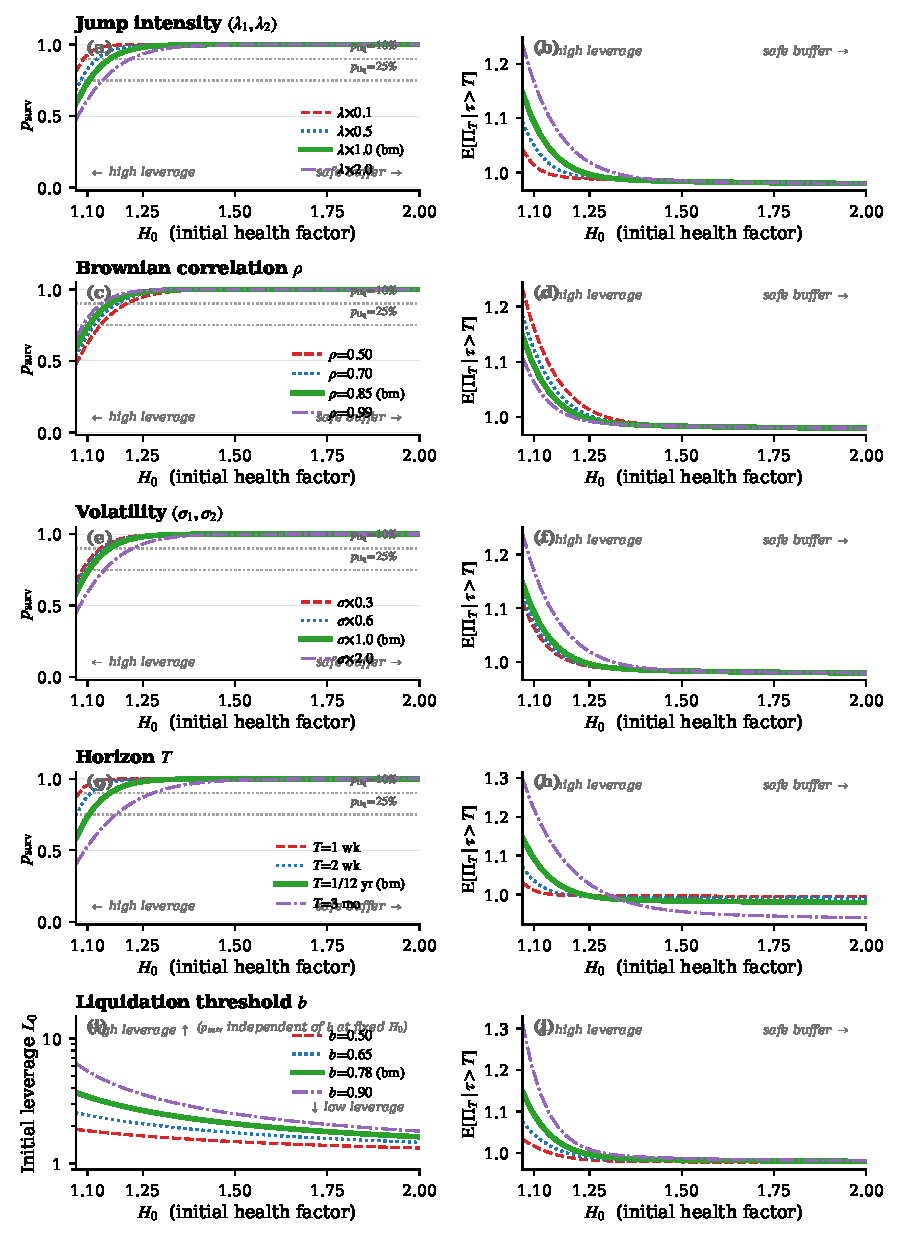
\includegraphics[width=0.95\linewidth]{fig_sensitivity_merged.pdf}
\caption{Left: survival probability (rows~a--d) and initial leverage $L_0$ (row~e, log scale) versus
$H_0$. Right: conditional mean $\E[\Pi_T\mid\tau>T]$. Each row varies one parameter, others at
Table~\ref{tab:num-params}; the heavier solid line is the benchmark. $H_0\in[1.068,2.000]$, 40
points per curve.}
\label{fig:sensitivity}
\end{figure}

% ============================================================
\section{Liquidation Recovery, Overshoot and Log Wealth}\label{sec:recovery}
% ============================================================

This section supplies $R_\tau$ in \eqref{eq:wealth} under the protocol's liquidation convention, at
the cost of one additional Laplace inversion per moment order and with the barrier system
unchanged. The same objects then give the law of the overshoot, the probability of bad debt and
the expected log of terminal wealth.

\subsection{Recovery at the barrier}
A liquidator repays debt and seizes collateral worth $(1+\ell)$ times the repayment, $\ell$ being the
liquidation bonus (Aave v3 Ethereum: $0.05$ for WETH, $0.045$ for major stablecoins, $0.05$--$0.075$
for wrapped BTC). Full repayment leaves $R_\tau=V_{1,\tau}-(1+\ell)V_{2,\tau}$. On a continuous
crossing $V_{2,\tau}=b\,V_{1,\tau}$, so
\begin{equation}\label{eq:recovery}
R_\tau \;=\; V_{2,\tau}\,\frac{1-b(1+\ell)}{b},
\end{equation}
positive when $\ell<1/b-1$ ($0.282$ at $b=0.78$). Writing recovery through the \emph{debt} leg makes
it proportional to $e^{X_{2,\tau}}$, the factor the framework already tilts by.

\begin{remark}[Continuous-crossing approximation]\label{rem:overshoot}
A downward jump can carry $H$ strictly below one, leaving less recovery than \eqref{eq:recovery},
possibly negative (bad debt). Equation~\eqref{eq:recovery} is therefore an upper bound;
Section~\ref{sec:overshoot} computes the exact value.
\end{remark}

\subsection{The first-passage transform}
We need $\E[e^{kX_{2,\tau}}\one_{\{\tau\le T\}}]$ for $k=1,2$. Since
$\exp(kX_{2,t}-t\Psi_k)$, $\Psi_k:=\Psi(0,-ik)$, is a martingale, changing measure on $\F_\tau$
gives $\E[e^{kX_{2,\tau}}\one_{\{\tau\le T\}}]=\E^{(k)}[e^{\Psi_k\tau}\one_{\{\tau\le T\}}]$, with
Laplace transform
\begin{equation}\label{eq:fp-transform}
\int_0^\infty e^{-qT}\,\E\!\left[e^{kX_{2,\tau}}\one_{\{\tau\le T\}}\right]\diff T
=\frac{1}{q}\Bigl(1-(q-\Psi_k)\,\widehat p^{\,(k)}_{\mathrm{surv}}(q-\Psi_k)\Bigr),
\qquad q>\Psi_k,
\end{equation}
where $\widehat p^{\,(k)}_{\mathrm{surv}}$ is the survival transform of
equation~\eqref{eq:survival-transform} under the $k$-tilted dynamics. Because $\Pi_T$ and
$R_\tau\one_{\{\tau\le T\}}$ live on disjoint events,
\begin{equation}\label{eq:wealth-moments}
\E[W_T]=\E[\Pi_T]+\E[R_\tau\one_{\{\tau\le T\}}],
\qquad
\E[W_T^2]=\E[\Pi_T^2]+\E[R_\tau^2\one_{\{\tau\le T\}}].
\end{equation}
At $k=0$, \eqref{eq:fp-transform} returns $p_{\mathrm{liq}}$ and agrees with
equation~\eqref{eq:survival-transform} to $1.7\times10^{-11}$.

Recovery is material. At $H_0=1.16$ ($p_{\mathrm{liq}}=0.10$) it raises mean terminal wealth from
$0.927$ to $0.981$ and cuts its variance from $0.127$ to $0.053$ by removing the total-loss atom at
zero. It matters for every levered buffer, but not for the break-even of
Section~\ref{sec:sizing}, which is set at zero debt, where liquidation vanishes.

\subsection{Exact recovery under jump overshoot}\label{sec:overshoot}
With the actual leg values at liquidation and $h_\tau:=h_0+Z_\tau\le0$ (zero at a continuous
crossing),
\begin{equation}\label{eq:recovery-exact}
R_\tau \;=\; V_{2,\tau}\!\left(\frac{e^{h_\tau}}{b}-(1+\ell)\right),
\end{equation}
which is smaller than \eqref{eq:recovery} whenever $h_\tau<0$. Rather than integrating against the
(exponential-mixture) overshoot density, we note that per unit initial equity
\begin{equation}\label{eq:joint-hit}
R_\tau=A\,e^{X_{1,\tau}}-B\,e^{X_{2,\tau}},
\qquad
\mathrm{Hit}(a_1,a_2):=\E\!\left[e^{a_1X_{1,\tau}+a_2X_{2,\tau}}\one_{\{\tau\le T\}}\right],
\end{equation}
with $A=H_0/(H_0-b)$ and $B=(1+\ell)b/(H_0-b)$, so $\E[R_\tau\one]=A\,\mathrm{Hit}(1,0)-B\,\mathrm{Hit}(0,1)$
and $\E[R_\tau^2\one]=A^2\mathrm{Hit}(2,0)-2AB\,\mathrm{Hit}(1,1)+B^2\mathrm{Hit}(0,2)$. The tilted
first-passage law already integrates over the landing point, so overshoot is captured exactly.
Tilting by $\exp(a_1X_{1,t}+a_2X_{2,t}-t\Psi_{\mathrm{M}}(a_1,a_2))$, with
$\Psi_{\mathrm{M}}(a_1,a_2):=\log\E[e^{a_1X_{1,1}+a_2X_{2,1}}]$, gives
\begin{equation}\label{eq:joint-hit-transform}
\int_0^\infty e^{-qT}\,\mathrm{Hit}(a_1,a_2)\,\diff T
=\frac1q\Bigl(1-(q-\Psi_{\mathrm{M}})\,\widehat p^{\,(a_1,a_2)}_{\mathrm{surv}}(q-\Psi_{\mathrm{M}})\Bigr),
\qquad q>\Psi_{\mathrm{M}}(a_1,a_2),
\end{equation}
where $\widehat p^{\,(a_1,a_2)}_{\mathrm{surv}}$ is the survival transform under the
$(a_1,a_2)$-tilted dynamics of $Z$, with exponent
$\psi_Z^{(a_1,a_2)}(s)=\Psi_{\mathrm{M}}(a_1+s,a_2-s)-\Psi_{\mathrm{M}}(a_1,a_2)$ and phase rates
$r_{1,+}=1/\eta_{1,+}-a_1$, $r_{1,-}=1/\eta_{1,-}+a_1$, $r_{2,+}=1/\eta_{2,-}+a_2$,
$r_{2,-}=1/\eta_{2,+}-a_2$; $(a_1,a_2)=(0,k)$ recovers Lemma~\ref{lem:psiZk}. The barrier system
stays $3\times3$. $\mathrm{Hit}(0,k)$ reproduces \eqref{eq:fp-transform} to $6\times10^{-14}$ and
$\mathrm{Hit}(0,0)$ reproduces $1-p_{\mathrm{surv}}$ to $3\times10^{-11}$; against an MC recording
leg values at the crossing step, all five moments agree up to a discretisation bias that shrinks with
the step count.

At the headline calibration's jump sizes ($\eta\approx0.4$--$1.1\%$) the correction is small: at $H_0=1.16$ mean
recovery falls from $0.054$ to $0.052$ ($-3\%$) and wealth variance rises from $0.053$ to $0.054$.
To see when overshoot bites, Table~\ref{tab:overshoot} scales the jumps two ways. Design~A scales
the mean jump size by $s$ at fixed intensity, which multiplies jump variance by $s^2$ --- a far more
volatile market. The correction reaches $-59\%$ at $s=10$ and mean recovery turns negative at
$s=20$: the continuous formula reports positive recovery where the protocol absorbs bad debt. Design~B
also divides intensity by $s^2$, holding jump variance fixed --- genuinely rarer, larger jumps. The
correction is just as severe ($-49\%$ at $s=10$, and at $s=20$ mean recovery is zero). The driver is
jump size rather than jump variance: at fixed variance the correction still eliminates recovery,
while the headline jumps carry about three quarters of the spread variance yet give only $-3\%$
because each is small.
Throughout, $R_\tau$ is the signed residual equity; a non-recourse borrower receives $R_\tau^+$,
which differs from it only on bad-debt paths, whose probability Section~\ref{sec:overshoot-law}
gives in closed form. The headline
calibration produces its kurtosis from many small jumps (cf.\ the identification ridge of
\citealt{RamezaniZeng2007} and Appendix~\ref{sec:ecf-ident}), so there the correction is small. It is
not small under every calibration: the full-history daily fit of Appendix~\ref{sec:full-history},
whose jumps are fewer and larger ($\eta_{2,+}\approx3.2\%$), gives a correction of $-11\%$ at
$H_0=1.16$.

\begin{table}[ht]
\centering
\small
\begin{tabular}{lcccc}
\toprule
 & \multicolumn{2}{c}{Design A: variance $\propto s^2$} & \multicolumn{2}{c}{Design B: variance fixed} \\
\cmidrule(lr){2-3}\cmidrule(lr){4-5}
Jump scale $s$ & $\E[R_\tau]$ exact & rel.\ corr. & $\E[R_\tau]$ exact & rel.\ corr. \\
\midrule
$1\times$ (fitted)  & $0.052$ & $-3\%$  & $0.052$ & $-3\%$ \\
$3\times$           & $0.210$ & $-16\%$ & $0.047$ & $-11\%$ \\
$10\times$          & $0.167$ & $-59\%$ & $0.018$ & $-49\%$ \\
$20\times$          & $-0.089$ & $-120\%$ & $-0.000$ & $-103\%$ \\
\bottomrule
\end{tabular}
\caption{Exact mean recovery at $H_0=1.16$ and its correction relative to the continuous-crossing
value \eqref{eq:recovery}. The continuous-crossing \emph{expected} recovery still moves with
$p_{\mathrm{liq}}$: under Design~A $p_{\mathrm{liq}}$ rises from $0.10$ to $0.69$ (continuous mean
recovery $0.054\to0.451$); under Design~B it falls to $0.03$ ($\to0.019$). Script
\texttt{overshoot\_table.py}.}
\label{tab:overshoot}
\end{table}

\subsection{The overshoot law and the probability of bad debt}\label{sec:overshoot-law}
The joint hitting moments integrate over the landing point without exposing it. The landing point
itself has a simple law. Write $u:=-h_\tau\ge0$ for the overshoot of the log health factor below the
barrier.

\begin{proposition}[Overshoot law]\label{prop:overshoot-law}
For every $T$ there are weights $P_0,P_1,P_2\ge0$, with $P_0+P_1+P_2=p_{\mathrm{liq}}(T)$, such that
for every bounded measurable $f$
\begin{equation}\label{eq:overshoot-law}
\E\!\left[f(u)\,\one_{\{\tau\le T\}}\right]
= P_0\,f(0)+\sum_{i=1}^{2}P_i\int_0^\infty f(u)\,r_ie^{-r_iu}\,\diff u,
\qquad r_1=\frac1{\eta_{1,-}},\quad r_2=\frac1{\eta_{2,+}}.
\end{equation}
The weights solve the $3\times3$ system
$e^{jh_0}\mathrm{Hit}(j,-j)=P_0+P_1\,r_1/(r_1+j)+P_2\,r_2/(r_2+j)$ for $j=0,1,2$.
\end{proposition}
\proofref{proof:prop:overshoot-law}

\noindent
$Z$ reaches the barrier either continuously (the diffusion creeps across, $u=0$) or by a downward
jump, which is a down-jump of $X_1$ (rate $r_1$) or an up-jump of $X_2$ (rate $r_2$). By
memorylessness, the excess of a crossing jump over the distance to the barrier is exponential with
the rate of that jump, whatever the path before it \citep{Kou2002,KouWang2003}; Appendix~\ref{app:proofs}
makes this precise with the compensation formula. This gives \eqref{eq:overshoot-law}. Taking $f(u)=e^{-ju}$, with
$e^{-ju}=e^{jh_0}e^{jZ_\tau}$ and $\mathrm{Hit}$ from \eqref{eq:joint-hit-transform}, yields the
system. At the benchmark the weights reproduce the hitting moments at $j=5$ and $j=10$ to about
$10^{-10}$, which checks the structure independently.

Recovery is non-positive exactly when $u\ge u^\star:=-\log\bigl(b(1+\ell)\bigr)$ ($0.200$ at
$b=0.78$, $\ell=0.05$). On those paths the protocol absorbs bad debt and a non-recourse borrower ends
with nothing. Proposition~\ref{prop:overshoot-law} gives the bad-debt probability in closed form,
\begin{equation}\label{eq:bad-debt}
\P\!\left(R_\tau\le0,\ \tau\le T\right)=P_1e^{-r_1u^\star}+P_2e^{-r_2u^\star}.
\end{equation}
It is $1\times10^{-9}$ at $H_0=1.16$ under the headline calibration, where jumps are below one
percent, and $3\times10^{-4}$ under the full-history daily calibration.

\subsection{Expected log wealth}\label{sec:log-wealth}
Moments of every admissible order cover polynomial criteria. The log of wealth, which defines the
growth-optimal (Kelly) investor \citep{Kelly1956,MacLeanThorpZiemba2011}, is not polynomial, but it
is also within reach. Per unit equity, $\Pi_T=e^{X_{2,T}}(e^{h_T}-b)/(H_0-b)$ on survival and
$R_\tau=e^{X_{2,\tau}}(e^{-u}-c)/(H_0-b)$ on liquidation, with $c:=b(1+\ell)$. Since
$\log(e^{h}-b)=h-\sum_{n\ge1}(b^n/n)e^{-nh}$ for $h\ge0$,
\begin{equation}\label{eq:log-wealth}
\begin{aligned}
\E[\log W_T]={}&\E\!\left[(X_{2,T}+h_T)\one_{\{\tau>T\}}\right]
-\sum_{n\ge1}\frac{b^n}{n}\,e^{-nh_0}S(-n,n)-\log(H_0-b)\\
&+\E\!\left[X_{2,\tau}\one_{\{\tau\le T\}}\right]
+\E\!\left[\log(e^{-u}-c)\,\one_{\{\tau\le T\}}\right],
\end{aligned}
\end{equation}
where $S(a_1,a_2):=\E[e^{a_1X_{1,T}+a_2X_{2,T}}\one_{\{\tau>T\}}]$ is a killed joint moment. Its
Laplace transform is the tilted survival transform at $q-\Psi_{\mathrm M}(a_1,a_2)$, by the change of
measure behind \eqref{eq:joint-hit-transform} applied on $\F_T$. The linear terms are tilt
derivatives of $S$ and $\mathrm{Hit}$ at zero, and the last term is a one-dimensional integral
against \eqref{eq:overshoot-law}. The series converges geometrically because
$b\,e^{-h_T}\le b<1$ on survival. The tilt $(-n,n)$ is admissible only for $n<\min(1/\eta_{2,+},1/\eta_{1,-})$, which
caps the series under heavy jump tails. Since $\E[e^{-nh_T}\one_{\{\tau>T\}}]$ decreases in $n$, the
truncation error after $N$ terms is at most $\E[e^{-Nh_T}\one_{\{\tau>T\}}]\,b^{N+1}/((N+1)(1-b))$,
which is below $10^{-5}$ in every case reported. The last term of \eqref{eq:log-wealth} is taken
over paths without bad debt; the next paragraph treats the rest.

Two features matter. First, under the zero-payoff convention $\log W_T=-\infty$ on every liquidated
path, so a Kelly investor never levers; recovery is what makes the criterion usable. Second, on
bad-debt paths $W_T=0$ even with recovery, so strict Kelly is $-\infty$ at every levered buffer
whenever \eqref{eq:bad-debt} is positive. On those paths we replace $\log(e^{-u}-c)$ in \eqref{eq:log-wealth}
by $\log10^{-4}$, which floors wealth at $10^{-4}e^{X_{2,\tau}}/(H_0-b)$, and report
\eqref{eq:bad-debt} alongside. Kelly quantities below refer to this floored objective. The floor is
immaterial at the headline calibration and of order $10^{-3}$ in $\E[\log W_T]$ at the thinnest
buffer under the full-history one. Evaluating \eqref{eq:log-wealth} takes about $0.3$\,s per buffer. A
bridge-corrected Monte Carlo that records the exact leg values at liquidation agrees to within $1.6$
standard errors at $H_0\in\{1.07,1.16,1.30\}$, and as $h_0\to\infty$ the expression tends to
$\E[X_{1,T}]$ to $10^{-6}$.

% ============================================================
\section{Sizing on the Evaluation Map}\label{sec:sizing}
% ============================================================

The evaluation map is objective-independent. This section applies it to the sizing problem of
Section~\ref{sec:1d}: first under several decision rules at the benchmark drift, then by asking
what the answer depends on, and finally by checking against realised outcomes. The drift is the
input that matters, and it is kept outside the calibration throughout.

\subsection{Decision rules on the map}\label{sec:rules}
Three rules illustrate how the same outputs enter different preferences.
\emph{A liquidation budget} selects the largest initial leverage whose liquidation probability does
not exceed $\bar p$,
\begin{equation}\label{eq:rule-constrained}
\max_{h_0\in\mathcal H}\ L_0(h_0)\quad\text{subject to}\quad p_{\mathrm{liq}}(T,h_0)\le\bar p ;
\end{equation}
it needs only the survival probability and is the rule a risk desk would apply.
\emph{Mean--variance on terminal wealth}, \eqref{eq:Phi} with exact recovery, and \emph{Kelly},
$\max_{h_0}\E[\log W_T]$ (Section~\ref{sec:log-wealth}), trade expected wealth against risk.
A fourth, popular rule --- mean--variance on survival-conditional moments with a liquidation
penalty --- is not recommended: conditioning keeps only the paths that survived, so the
conditional mean rises as the buffer thins and the rule rewards leverage for a survivorship
artefact (Table~\ref{tab:results}).

\begin{table}[ht]
\centering
\small
\begin{tabular}{llccc}
\toprule
Rule & Parameter & $H_0$ & $L_0$ & $p_{\mathrm{liq}}$ \\
\midrule
Liquidation budget \eqref{eq:rule-constrained} & $\bar p=0.01$ & $1.281$ & $2.56$ & $0.010$ \\
 & $\bar p=0.05$ & $1.199$ & $2.86$ & $0.050$ \\
 & $\bar p=0.10$ & $1.160$ & $3.05$ & $0.100$ \\
 & $\bar p=0.20$ & $1.118$ & $3.31$ & $0.200$ \\
\midrule
Mean--variance on $W_T$ & $\alpha=0.5$ & --- & $2.19$ & --- \\
 & $\alpha=1$ & --- & $1.91$ & --- \\
 & $\alpha=2$ & --- & $1.40$ & --- \\
Kelly, $\E[\log W_T]$ & full & --- & $1.91$ & --- \\
 & half & --- & $1.45$ & --- \\
 & quarter & --- & $1.23$ & --- \\
\midrule
Any of the last six, no relative-drift view & --- & $\infty$ & $1$ & $0$ \\
\bottomrule
\end{tabular}
\caption{Selections on the benchmark map (sample drift $\nu=\mu_1-\mu_2=+0.103$ per year,
$T=1/12$). The budget rows maximise $L_0$ subject to $p_{\mathrm{liq}}\le\bar p$. The
mean--variance and Kelly rows search $30$ debt levels over the full buffer range plus the
unlevered position, with exact recovery; fractional Kelly holds the stated fraction of the Kelly
debt. The last row sets the relative price drift to zero, so that $\nu$ equals the net carry. Scripts \texttt{decision\_rules.py} and
\texttt{breakeven\_drift.py}.}
\label{tab:rules}
\end{table}

The selections differ widely across rules (Table~\ref{tab:rules}), as an objective-independent map
should allow. Two features matter for what follows. First, the budget rule is robust to the drift,
because over a month the liquidation probability is driven mainly by volatility and jumps: with a
$5\%$ budget it selects $L_0$ between $2.66$ and $3.04$ for any drift from $-0.5$ to $+0.6$ per year.
The mean--variance and Kelly selections are driven by the drift: at the sample drift they lever
moderately, and without a relative-drift view every one of them selects the unlevered position. Second, the search must include the unlevered position. A grid capped at a finite buffer,
such as $H_0\le2$ ($L_0=1.64$), reports its cap whenever the true optimum is unlevered, which
manufactures an apparent interior optimum. Fractional Kelly, the usual response to an uncertain
drift \citep{MacLeanThorpZiemba2011}, scales the Kelly debt down but does not change whether to
borrow at all: a fraction of zero debt is zero. The rest of this section therefore asks at which
drift leverage starts to pay, and whether the data can tell.

\subsection{Break-even drift views}
Write $x:=n_2S_{2,0}=b/(e^{h_0}-b)$ for the debt per unit of equity, so that $x=0$ is the unlevered
position and $L_0=1+x$. Leverage improves on the unlevered position exactly when the first unit of
debt does, and that is a closed-form question. As $x\to0$ the buffer becomes infinite and the
liquidation probability vanishes, so $W_T=(1+x)e^{X_{1,T}}-x\,e^{X_{2,T}}$ to first order, and
\begin{equation}\label{eq:breakeven}
\left.\frac{\diff\Phi}{\diff x}\right|_{x=0}
=\bigl(\E e^{X_{1,T}}-\E e^{X_{2,T}}\bigr)-\alpha\,\mathrm{Cov}\bigl(e^{X_{1,T}},\,e^{X_{1,T}}-e^{X_{2,T}}\bigr),
\qquad
\left.\frac{\diff\,\E[\log W_T]}{\diff x}\right|_{x=0}=1-\E\,e^{X_{2,T}-X_{1,T}},
\end{equation}
for mean--variance \eqref{eq:Phi} and for Kelly. All terms are joint exponential moments
$e^{T\Psi_{\mathrm M}(a_1,a_2)}$. The \emph{break-even drift view} $\nu^\star$ is the spread drift
$\nu=\mu_1-\mu_2$ (price growth plus net carry) at which the derivative vanishes, holding the level
$\mu_2$ at its sample value. Without liquidation both objectives are concave in $x$ (mean--variance
is a concave quadratic, $\log$ a concave function of an affine one), so the sign of the derivative at
$x=0$ decides between the unlevered position and some leverage. Liquidation breaks this argument, so
we check it numerically: a search over $30$ debt levels spanning the full buffer range, from
$x=10^{-3}$ ($H_0\approx781$) to the origination maximum, with exact recovery and the floored Kelly
objective of Section~\ref{sec:log-wealth}, confirms the switch at $\nu^\star$ for every objective
and calibration.

For Kelly the condition $\E e^{X_{2,T}-X_{1,T}}=1$ is $\Psi_{\mathrm M}(-1,1)=0$, which does not
depend on $T$ and, with independent jump processes, solves in closed form:
\begin{equation}\label{eq:kelly-breakeven}
\nu^\star_{\mathrm{Kelly}}=\underbrace{\sigma_1^2-\rho\sigma_1\sigma_2}_{\text{diffusion}}
+\underbrace{\lambda_1\bigl[M_1(1)+M_1(-1)-2\bigr]}_{\text{WBTC jumps}},
\qquad M_1(s)=\frac{p_1}{1-s\eta_{1,+}}+\frac{1-p_1}{1+s\eta_{1,-}}.
\end{equation}
The break-even views are small (Table~\ref{tab:thresholds}): about $0.4$--$1.6\%$ per year under the
headline calibration and $2.4$--$11\%$ under the full-history ones, close to linear in $\alpha$, with
Kelly near $\alpha=1$. Equation~\eqref{eq:kelly-breakeven} says why. The diffusion part is negative,
because WBTC is the less volatile leg ($\sigma_1<\rho\sigma_2$): at the margin, shorting WETH
against WBTC reduces diffusive risk. The break-even is positive only through WBTC's own jumps, which
the short leg does not hedge: $-0.004+0.012$ under the headline calibration, $-0.017+0.065$ under the
full-history daily one and $-0.009+0.054$ under the 2024 one. The second term rests on the
jump parameters, which the data identify weakly (Appendix~\ref{sec:calibration}), and a common jump
component, which the model excludes, would reduce it by the covariance of the two legs' jumps.
Section~\ref{sec:realised} shows that this is the case in the data: the realised break-even of
WBTC/WETH is negative. With no
relative-drift view at all, $\nu$ equals the net carry ($\approx-2.5\%$), below every break-even, so
the unlevered position is optimal for every objective. Above $\nu^\star$ the optimal leverage rises
quickly with the view (Figure~\ref{fig:buffer-drift}).

\begin{table}[ht]
\centering
\small
\begin{tabular}{lccccc}
\toprule
Calibration & model $\bar\sigma_Z$ & $\alpha=0.5$ & $\alpha=1$ & Kelly & $\alpha=2$ \\
\midrule
Headline, 4h, 2026-03 to 08 ($0.38$ y) & $0.335$ & $+0.004$ & $+0.008$ & $+0.008$ & $+0.016$ \\
Full history, daily ($3.7$ y) & $0.478$ & $+0.027$ & $+0.054$ & $+0.048$ & $+0.110$ \\
2024 onward, 4h ($2.8$ y) & $0.485$ & $+0.024$ & $+0.049$ & $+0.045$ & $+0.099$ \\
\bottomrule
\end{tabular}
\caption{Break-even spread-drift views $\nu^\star$ (per year, price growth plus net carry): the
unlevered position is optimal below $\nu^\star$ and some leverage above it, for mean--variance on
terminal wealth with exact recovery and for Kelly, from \eqref{eq:breakeven}, with $\mu_2$ at the
sample level of the matching window (the full-history one for the 2024 calibration). ``Model
$\bar\sigma_Z$'' is the calibrated total (diffusion plus jump) spread volatility. Script
\texttt{breakeven\_drift.py}.}
\label{tab:thresholds}
\end{table}

\begin{figure}[ht]
\centering
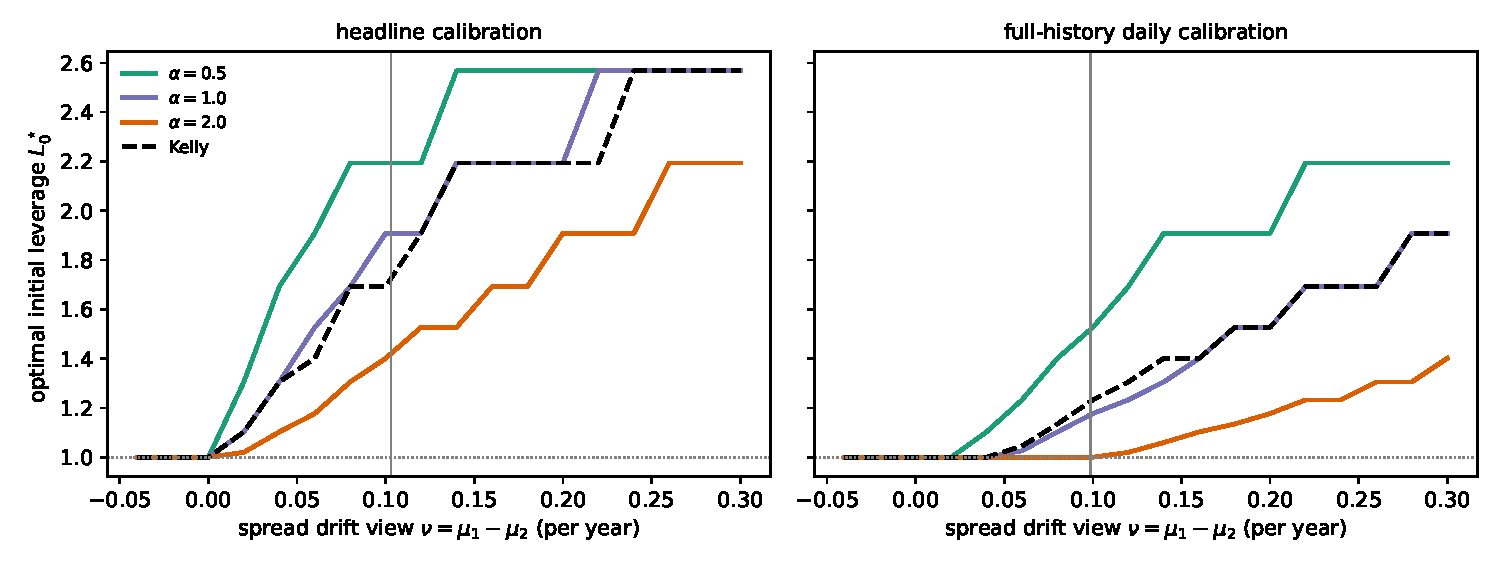
\includegraphics[width=0.95\linewidth]{fig_buffer_drift.pdf}
\caption{Optimal initial leverage $L_0^\star$ against a drift view $\nu=\mu_1-\mu_2$, mean--variance
on terminal wealth ($\alpha=0.5,1,2$) and Kelly, exact recovery, over the full buffer range. Left:
headline calibration; right: full-history daily calibration. The optimum is unlevered ($L_0^\star=1$)
below the break-even view and rises quickly above it. The vertical line marks the sample drift of
each window. The optimum is located on $30$ debt levels plus the unlevered position, hence the steps. Script
\texttt{breakeven\_drift.py}.}
\label{fig:buffer-drift}
\end{figure}

\subsection{What the data say about the drift}
The spread drift has two parts, $\nu=\nu_{\mathrm{price}}+c$. The net carry $c=r_s-r_b$ is observed
on-chain, about $-2.5\%$ per year for WBTC/WETH. The relative price growth $\nu_{\mathrm{price}}$ is
the expected outperformance of WBTC over WETH, and it is estimated poorly at any sampling
frequency, because the standard error of a drift depends only on calendar length
\citep{Merton1980}, so, as in Section~\ref{sec:numerical}, we use sample means. The headline window gives
$\nu=+0.10$ (price $+0.13$, carry $-0.025$) with a Newey--West standard error of $0.34$; the full
$3.7$-year daily history gives $\nu=+0.10$ (price $+0.13$, carry $-0.03$) with a Newey--West and
block-bootstrap standard error of $0.19$; and the yearly estimates of $\nu_{\mathrm{price}}$ range
from $-0.16$ to $+0.34$ with standard errors of $0.3$--$0.5$. Both point estimates lie above every
headline break-even and above most full-history ones, and at them the optimal leverage is moderate
($1.4$--$2.2$ under the headline calibration, $1.0$--$1.5$ under the full-history ones). But the
standard errors are several times the gap between estimate and break-even: telling $+0.10$ from the
full-history Kelly break-even of $+0.05$ at two standard errors would need a standard error of
$0.025$, about two centuries of data. Both reserves accept collateral and borrowing, so the book can
also be held the other way round. Reversing the legs flips the sign of $\nu_{\mathrm{price}}$ and
changes the carry: over the full history, WETH collateral against WBTC debt has
$\nu_{\mathrm{price}}=-0.13$ and $c=+1.1\%$, so $\nu=-0.11$. Its Kelly break-even, the mirror image
of \eqref{eq:kelly-breakeven} with the legs exchanged, is $+0.10$ to $+0.19$ across the calibrations
and has a positive diffusion part, because WETH is the more volatile leg; the reversed book is thus
far from paying, even though WETH's higher liquidation threshold ($0.83$ against $0.78$) would allow
more leverage. A
relative-drift view therefore chooses the orientation as well as the buffer.

A carry-anchored Bayesian layer turns this into a probability. Take $\nu\sim\mathcal N(c,0.20^2)$,
the view that relative prices have no predictable drift, and update it with the sample estimate.
The posterior probability that leverage pays, $\P(\nu>\nu^\star)$, is $48$--$51\%$ for every objective
under the headline calibration and $30$--$54\%$ under the full-history ones, treating $\nu^\star$ as
known. Under a flat prior, which takes the sample estimate at face value, it is $60$--$62\%$ and
$48$--$65\%$. Either way the data leave the question close to open. Maximising the posterior
expectation of $\E[\log W_T]$ (Bayes--Kelly) has an exact rule at the margin: with posterior
$\mathcal N(m,s^2)$, lever if and only if $m>\nu^\star_{\mathrm{Kelly}}+\tfrac12Ts^2$. The variance
term is small ($0.001$ at the headline posterior), so the rule is decided by the posterior mean. The
carry-anchored prior pulls it to $+0.008$ (headline) and $+0.039$ (full history), just below the
thresholds $+0.009$ and $+0.046$--$0.049$, and Bayes--Kelly selects the unlevered position under all
three calibrations. Under the flat prior $m=\hat\nu\approx0.10$ and it levers. The unlevered choice
therefore reflects the prior's shrinkage toward zero relative drift, not estimation risk as such. Out of sample, the fitted ECF drift also worsens the map's
liquidation forecasts relative to setting $\nu_{\mathrm{price}}=0$ (Appendix~\ref{sec:full-history}).

\subsection{Did leverage pay? A realised backtest}\label{sec:realised}
The break-even rule says when leverage pays; whether it did is a question for realised data, and
one that needs no model. We replay every pair of the pre-registered cross-section
(Appendix~\ref{sec:carry-crosssection}; $37$ pairs) hour by hour on the Aave v3 Ethereum history: oracle-implied prices, the collateral's
supply rate and the debt's borrow rate. Windows run from the first hour at which both reserves are
live (27 January 2023 for the original reserves, up to 23 September 2024 for cbBTC) to 13 October
2026. Equity is in dollars. At each roll date the book is reset to initial leverage $L_0$; between
rolls interest accrues on both legs, and whenever the health factor falls below one at an hourly
mark a keeper repays half the debt (all of it below $0.95$) and seizes collateral worth the repayment
plus the reserve's bonus, as on Aave v3. The benchmark holds the collateral unlevered. Rolled books
are averaged over four roll phases and buy-and-hold books over four start dates $120$ days apart.
Standard errors are Newey--West on daily excess log returns ($60$-day lag).

\begin{table}[ht]
\centering
\small
\begin{tabular}{lcccc}
\toprule
Roll horizon & $L_0=1.25$ & $L_0=1.5$ & $L_0=2$ & $L_0=3$ \\
\midrule
1 day & $-0.038$ \ (4) & $-0.102$ \ (4) & $-0.287$ \ (3) & $-0.768$ \ (0) \\
30 days & $-0.042$ \ (4) & $-0.113$ \ (4) & $-0.331$ \ (4) & $-0.994$ \ (1) \\
365 days & $-0.008$ \ (5) & $-0.112$ \ (5) & $-0.559$ \ (3) & $-0.889$ \ (2) \\
Buy and hold & $-0.017$ \ (12) & $-0.036$ \ (12) & $-0.303$ \ (10) & $-0.451$ \ (7) \\
\bottomrule
\end{tabular}
\caption{Realised excess log growth per year of the levered over the unlevered book: median over
the $37$ pairs, with the number of pairs in which leverage paid in parentheses. Aave v3 liquidation
rules, current reserve parameters, no trading costs. Script \texttt{realised\_backtest.py}.}
\label{tab:realised}
\end{table}

\begin{figure}[ht]
\centering
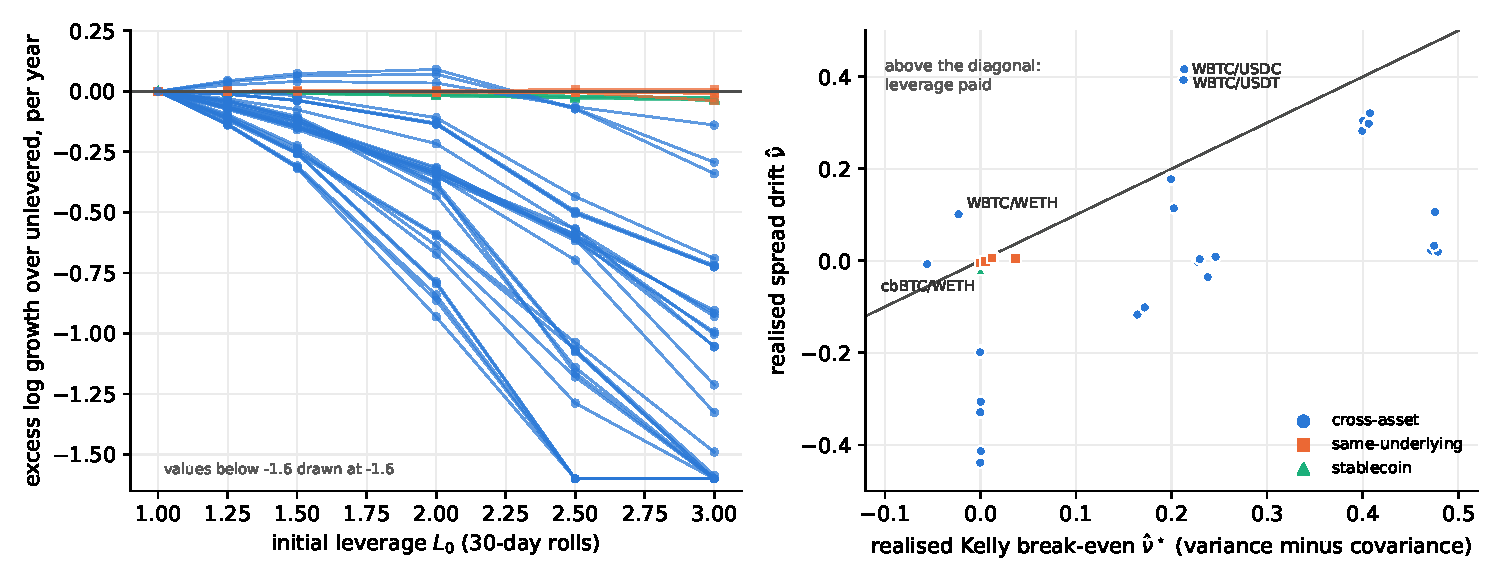
\includegraphics[width=0.95\linewidth]{fig_realised_backtest.pdf}
\caption{Left: realised excess log growth against initial leverage, $30$-day rolls, one line per
pair. Right: realised spread drift $\hat\nu$ against the realised Kelly break-even $\hat\nu^\star$,
both from daily gross returns including interest; above the diagonal a little leverage paid.
Script \texttt{fig\_realised\_backtest.py}.}
\label{fig:realised-backtest}
\end{figure}

Leverage rarely paid (Table~\ref{tab:realised}, Figure~\ref{fig:realised-backtest}). At $L_0=1.25$
it beat the unlevered book in $4$ of $37$ pairs --- WBTC against USDC, USDT and WETH, and cbBTC against
WETH, all books long BTC in a window in which BTC rose $3.6$-fold and doubled against ETH --- and
in none significantly. Of $1{,}332$ pair, leverage and horizon combinations, one has $t>2$ and $338$
have $t<-2$; the four stablecoin pairs lose significantly at every leverage up to $3\times$ and every
horizon, because their net carry over the window is negative and nearly deterministic. Losses grow quickly with
leverage, through volatility drag at every horizon and through liquidations once the book is left
for a week or more: from $L_0=2.5$ most pairs are liquidated at least once at those horizons, and a
book rolled at the maximum LTV loses in every pair. A $10$\,bp trading cost per reset leaves these
numbers almost unchanged, and so does the paper's full-liquidation convention for rolled books up to
$L_0=2$; for buy-and-hold at high leverage it loses less than Aave's partial liquidations, because
after one liquidation the residual is held unlevered. Rolling more often does not help: at low leverage the excess is about the same from one
day to a year. Buy and hold does better, because a static book's leverage falls as it gains and it
avoids the volatility drag of re-levering, but it still loses in most pairs. Nor is short-term profitability a matter
of calendar time: at $L_0=2$ and $30$-day rolls, $17\%$ of cross-asset pair-years were positive, almost
all of them BTC-long books in 2023--24 or ETH-long books against dollars in 2023, and none of the $29$
in 2025. The window is one cycle --- a bull market
to the 2025 peaks, then a decline of $53\%$ for BTC and $68\%$ for ETH to mid-2026 --- with one
dominant cross-asset trend, so these numbers describe this history, not a law. A simple ex-ante rule
that levers to $2\times$ for a month only after a positive trailing-year spread return lost less than
always levering in $29$ pairs but beat the unlevered book in only $5$.

The realised break-even confirms the rule and exposes the model. For a daily-rolled book the
marginal log growth of the first unit of debt is $\E[1-R_2/R_1]$ in daily gross returns, so leverage
pays at the margin if and only if $\hat\nu>\hat\nu^\star$, the realised counterpart of
\eqref{eq:kelly-breakeven}; this is a first-order identity, and it sorts all $37$ pairs correctly.
Its value lies in the comparison with the model. For WBTC/WETH, $\hat\nu^\star=-0.023$ (daily;
$-0.026$ four-hourly), against the full-history model's $+0.048$. The legs' realised correlation is
$0.81$, and on $85\%$ of the days with a three-standard-deviation move in either leg both legs move
by more than one and a half standard deviations in the same direction; the calibrated model, whose jumps are independent, has correlation $0.50$. With only Brownian
correlation to carry co-movement, the fit cannot match the common jumps: it understates both legs'
variances (WBTC $0.15$ against $0.21$ per year) and, by much more, their covariance ($0.11$ against
$0.24$), so the spread variance is overstated ($0.23$ against $0.14$) and the break-even, collateral
variance minus covariance, turns positive. The same overstatement inflates the model's liquidation
probabilities and is consistent with their excess over realised frequencies out of sample
(Appendix~\ref{sec:full-history}). A common jump component --- a third Poisson process
moving both legs, with double-exponential marks so that the spread's jumps stay in the
mixed-exponential class of Section~\ref{sec:resolvent}, at the cost of more phases and a larger
barrier system --- is therefore the most consequential extension of the model.

\subsection{A decision-theoretic extension}\label{sec:extension}
These results suggest a separate treatment of the sizing problem, which we leave to future work.
Its question is whether a leveraged position of this kind can be sized from data at all. Four
pieces would be needed.
\emph{(i)} A preference-free break-even: the killed law of $Z_T$ and the overshoot law of
Proposition~\ref{prop:overshoot-law} determine the full distribution of $W_T$, so one can find the
drift views below which the unlevered position second-order stochastically dominates every levered
one. Below that view every risk-averse investor agrees, not only the objectives above.
\emph{(ii)} The CRRA family, which extends Section~\ref{sec:log-wealth} by the binomial series in
place of the logarithmic one, with the same tilted moments.
\emph{(iii)} An explicit account of estimation risk in the tradition of
\citet{Barberis2000}, \citet{KanZhou2007} and \citet{DeMiguel2007}, and of fractional Kelly
\citep{MacLeanThorpZiemba2011}, with the break-even view $\nu^\star$ as the decision rule: lever only
if one's relative-drift view, including carry, exceeds it, and size the position by the posterior
rather than the point estimate.
\emph{(iv)} A repeated, monthly-rolled version in which liquidation is partial ruin and long-run
growth is the natural criterion.

% ============================================================
\section{Conclusion}\label{sec:conclusion}
% ============================================================

We derive a semi-analytic evaluation map for leveraged DeFi long--short positions under
liquidation and jump risk. The initial log health factor reduces the holdings to one parameter, an
exponential change of measure reduces each admissible payoff moment to a killed expectation of the
log price ratio, and under Kou dynamics three barrier conditions give a $3\times3$ resolvent system
for every moment order. Bivariate tilts of the same system give the exact liquidation recovery under
jump overshoot, the overshoot law and the probability of bad debt, and the expected log of terminal
wealth. The map is noise-free, fast and validated against an accuracy-matched simulator; out of
sample its one-month liquidation probabilities lie above realised frequencies, systematically so for
some predictors.

Applied to sizing, the map turns any of the usual objectives into a one-dimensional search, and the
selection moves with the objective, its risk parameters and the loss convention. Beneath that
variety sits one quantity: the closed-form break-even drift above which the first unit of debt pays,
about $0.4$--$11\%$ per year depending on risk attitude and calibration. The sample drift lies near
or above it, but with standard errors several times the gap, so the data cannot tell an investor
whether to lever. Ex post, leverage rarely paid: replayed under Aave's liquidation rules over
2023--2026, it beat the unlevered position in $4$ of $37$ pairs at modest leverage and in none
significantly. The realised break-evens also disagree with the model's for WBTC/WETH, because the
model's independent jumps cannot reproduce the legs' common jumps.

The principal output is therefore not a leverage number but the map itself, which evaluates a buffer
under a stated drift view or stress scenario and is the input any sizing rule needs. The most
consequential extension is a common jump component. Others are a decision-theoretic treatment of
sizing under drift uncertainty (Section~\ref{sec:extension}), an endogenous utilization process in
place of the exogenous rate regime of Appendix~\ref{app:carry}, the stochastic control problem of
Remark~\ref{rem:dynamic}, and a market-impact channel that makes the liquidation bonus endogenous
in the overshoot regime.

\appendices

% ============================================================
\section{Killing at the Barrier and Downward-Phase Corrections}
\label{app:downward-phases}
% ============================================================

Section~\ref{sec:resolvent} uses only the generator $\mathcal L^{(k)}$ from
Lemma~\ref{lem:psiZk}, with a killed expectation extended by zero below the barrier. This
appendix records how that convention changes the downward jump integrals and derives the
three rows of the barrier system \eqref{eq:barrier-system}.

\subsection{Phase Operators and Zero Extension}

\begin{definition}[Phase operators]\label{def:phase-ops}
For $j=1,2$, the phase operators associated with the tilted jump kernels of $Z$ under
$\P^{(k)}$ are
\[
K_{j,+}^{(k)}[f](x)
:=
\int_0^\infty f(x+y)r_{j,+}^{(k)}e^{-r_{j,+}^{(k)}y}\,\diff y,
\qquad
K_{j,-}^{(k)}[f](x)
:=
\int_0^\infty f(x-y)r_{j,-}^{(k)}e^{-r_{j,-}^{(k)}y}\,\diff y.
\]
For any complex $\gamma$ with
$\Rea(\gamma)<r_{j,+}^{(k)}$ and $\Rea(\gamma)>-r_{j,-}^{(k)}$, direct integration gives
\begin{equation}\label{eq:phase-on-exp}
K_{j,+}^{(k)}[e^{\gamma\cdot}](x)
=
\frac{r_{j,+}^{(k)}}{r_{j,+}^{(k)}-\gamma}e^{\gamma x},
\qquad
K_{j,-}^{(k)}[e^{\gamma\cdot}](x)
=
\frac{r_{j,-}^{(k)}}{r_{j,-}^{(k)}+\gamma}e^{\gamma x}.
\end{equation}
\end{definition}
This phase construction originates in \citet{KouWang2003} for first-passage problems under
the double-exponential model and is used by \citet{Sepp2004} to reduce barrier pricing to a
finite linear system.

The tilted phase intensities are
\begin{equation}\label{eq:tilted-intensities}
\lambda_{1,+}^{(k)}=\lambda_1p_1,
\quad
\lambda_{1,-}^{(k)}=\lambda_1(1-p_1),
\quad
\lambda_{2,+}^{(k)}=\frac{\lambda_2(1-p_2)}{1+k\eta_{2,-}},
\quad
\lambda_{2,-}^{(k)}=\frac{\lambda_2p_2}{1-k\eta_{2,+}}.
\end{equation}
Using Definition~\ref{def:phase-ops}, the full-line action of the generator is
\begin{equation}\label{eq:generic-generator}
\mathcal L^{(k)}f(x)
=\mu_Z^{(k)}f'(x)+\frac{\sigma_Z^2}{2}f''(x)
+\sum_{a=1}^2\lambda_{a,+}^{(k)}\bigl(K_{a,+}^{(k)}[f](x)-f(x)\bigr)
+\sum_{d=1}^2\lambda_{d,-}^{(k)}\bigl(K_{d,-}^{(k)}[f](x)-f(x)\bigr).
\end{equation}
Applying \eqref{eq:phase-on-exp} recovers the exponential symbol
\eqref{eq:generator-eigen}.

Now let $f$ be defined on the alive half-line $x>0$ and let
$\bar f=f\one_{(0,\infty)}$ be its zero extension. Upward jumps remain in the alive region,
whereas a downward jump of size $y\ge x$ lands in the absorbing region. Consequently,
\begin{equation}\label{eq:killed-downward-operator}
K_{d,-}^{(k)}[\bar f](x)
=K_{d,-}^{(k),D}[f](x)
:=\int_0^x f(x-y)r_{d,-}^{(k)}e^{-r_{d,-}^{(k)}y}\,\diff y,
\qquad x>0.
\end{equation}
Substitution into \eqref{eq:generic-generator} gives
\begin{equation}\label{eq:zero-extended-generator}
\begin{aligned}
\mathcal L^{(k)}[\bar f](x)
={}&\mu_Z^{(k)}f'(x)+\frac{\sigma_Z^2}{2}f''(x)
+\sum_{a=1}^2\lambda_{a,+}^{(k)}
  \bigl(K_{a,+}^{(k)}[f](x)-f(x)\bigr)\\
&+\sum_{d=1}^2\lambda_{d,-}^{(k)}
  \bigl(K_{d,-}^{(k),D}[f](x)-f(x)\bigr),
\qquad x>0.
\end{aligned}
\end{equation}
Thus killing changes the arguments on which $\mathcal L^{(k)}$ acts, not the identity of the
generator. Equation~\eqref{eq:zero-extended-generator} is the standard zero-extension
construction for a L\'evy process killed at an absorbing boundary.

\subsection{Downward-Phase Residual and Barrier Conditions}

\begin{lemma}[Truncated downward phase]\label{lem:truncated-phase}
For $r>0$, $\beta\in\mathbb C\setminus\{-r\}$, and $x>0$,
\begin{equation}\label{eq:truncated-phase}
\int_0^x e^{\beta(x-y)}r e^{-ry}\,\diff y
=\frac{r}{r+\beta}e^{\beta x}
-\frac{r}{r+\beta}e^{-rx}.
\end{equation}
No restriction $\Rea(\beta)>-r$ is needed, since the integral is over a finite interval.
\end{lemma}
\proofref{proof:lem:truncated-phase}

For a finite exponential sum $v(x)=\sum_{\beta\in\mathcal E}a_\beta e^{\beta x}$, define
the truncation-correction coefficient
\begin{equation}\label{eq:correction-functional}
\mathfrak C_r[v]
:=\sum_{\beta\in\mathcal E}a_\beta\frac{r}{r+\beta}.
\end{equation}
Then \eqref{eq:truncated-phase} gives
\begin{equation}\label{eq:truncated-decomposition}
K_{r,-}^{D}[v](x)
:=\int_0^x v(x-y)re^{-ry}\,\diff y
=\sum_{\beta\in\mathcal E}a_\beta\frac{r}{r+\beta}e^{\beta x}
-\mathfrak C_r[v]e^{-rx}.
\end{equation}
Combining \eqref{eq:zero-extended-generator} and
\eqref{eq:truncated-decomposition}, for exponents at which the upward integrals are finite
and which avoid the downward phase poles,
\begin{equation}\label{eq:zero-extension-residual}
\mathcal L^{(k)}[\bar v](x)
=\sum_{\beta\in\mathcal E}a_\beta\psi_Z^{(k)}(\beta)e^{\beta x}
-\sum_{d=1}^2\lambda_{d,-}^{(k)}
  \mathfrak C_{r_{d,-}^{(k)}}[v]e^{-r_{d,-}^{(k)}x},
\qquad x>0,
\end{equation}
where $\psi_Z^{(k)}$ is understood through the meromorphic continuation of its exponential
symbol outside the common full-line moment strip.

Apply \eqref{eq:zero-extension-residual} term by term to the interior ansatz
\eqref{eq:interior-ansatz}. Its forcing coefficients and characteristic-root equations give
\begin{equation}\label{eq:killed-residual}
(q-\mathcal L^{(k)})\widehat U_k(q,x)
=G_k(x)
+\sum_{d=1}^2\lambda_{d,-}^{(k)}
  \mathfrak C_{r_{d,-}^{(k)}}[\widehat U_k(q,\cdot)]
  e^{-r_{d,-}^{(k)}x}.
\end{equation}
When the two downward rates are distinct, the residual exponentials are linearly
independent, so the interior equation holds if and only if both correction coefficients
vanish. Since $\sigma_Z>0$, the lower boundary is regular for the Brownian component and
absorption also imposes the Dirichlet condition. The three conditions are therefore
\begin{equation}\label{eq:three-barrier-conditions}
\widehat U_k(q,0)=0,
\qquad
\mathfrak C_{r_{1,-}^{(k)}}[\widehat U_k(q,\cdot)]=0,
\qquad
\mathfrak C_{r_{2,-}^{(k)}}[\widehat U_k(q,\cdot)]=0.
\end{equation}
Substituting \eqref{eq:interior-ansatz} into \eqref{eq:three-barrier-conditions} gives
\[
\sum_{m=1}^3B_m^{(k)}
=-\sum_{j=0}^{k}\frac{d_{k,j}}{q-\psi_Z^{(k)}(j)},
\]
and, for $d=1,2$,
\[
\sum_{m=1}^3
\frac{r_{d,-}^{(k)}}{r_{d,-}^{(k)}+\gamma_{m+3}^{(k)}(q)}B_m^{(k)}
=-\sum_{j=0}^{k}\frac{d_{k,j}}{q-\psi_Z^{(k)}(j)}
  \frac{r_{d,-}^{(k)}}{r_{d,-}^{(k)}+j}.
\]
These are precisely the three rows of \eqref{eq:barrier-system}.

\begin{remark}[Coincident downward rates]\label{rem:coincident-rates}
If $r_{1,-}^{(k)}=r_{2,-}^{(k)}=:r$, the two downward kernels combine into a single phase.
The meromorphic symbol must first be reduced by cancelling the repeated phase factor;
otherwise clearing denominators introduces a spurious root at the pole $-r$. The reduced
characteristic equation has two genuine decaying roots, say
$\gamma_4^{(k)}(q),\gamma_5^{(k)}(q)$, and the
conditions $\widehat U_k(q,0)=0$ and
$\mathfrak C_r[\widehat U_k(q,\cdot)]=0$ give the $2\times2$ system
\[
\begin{pmatrix}
1&1\\[4pt]
\dfrac{r}{r+\gamma_4^{(k)}(q)}&\dfrac{r}{r+\gamma_5^{(k)}(q)}
\end{pmatrix}
\begin{pmatrix}B_1^{(k)}\\B_2^{(k)}\end{pmatrix}
=-
\begin{pmatrix}
\displaystyle\sum_{j=0}^{k}\frac{d_{k,j}}{q-\psi_Z^{(k)}(j)}\\[10pt]
\displaystyle\sum_{j=0}^{k}\frac{d_{k,j}}{q-\psi_Z^{(k)}(j)}\frac{r}{r+j}
\end{pmatrix}.
\]
Thus the $3\times3$ description applies to the generic distinct-rate regime; the
coincident-rate case is a genuine lower-dimensional phase model, not a singular generic
system.
\end{remark}

\clearpage

% ============================================================
\section{Empirical Calibration}\label{sec:calibration}
% ============================================================

\subsection{Estimator}\label{sec:ecf-estimator}

The model characteristic function over an observation interval $\Delta$ is available in closed form,
\begin{equation}\label{eq:model-cf}
\phi_\theta(u,v;\Delta)
=
\exp\!\bigl(\Delta\,\Psi_\theta(u,v)\bigr).
\end{equation}
Given $N$ bivariate log-returns $(r_{1,n},r_{2,n})$, with empirical characteristic function
\begin{equation}\label{eq:ecf}
\widehat{\phi}_N(u,v)
=
\frac{1}{N}\sum_{n=1}^N
\exp\!\bigl(i(u\,r_{1,n}+v\,r_{2,n})\bigr),
\end{equation}
we estimate $\theta$ by penalised ECF matching,
\begin{equation}\label{eq:ecf-objective}
\begin{aligned}
\widehat{\theta}
=
\arg\min_{\theta\in\Theta}\;
&\sum_{(u,v)\in\mathcal{G}}
w(u,v)
\,\bigl|\widehat{\phi}_N(u,v)-\phi_\theta(u,v;\Delta)\bigr|^2\\
&+\kappa_\lambda\sum_{i=1}^2\bigl(\log\lambda_i-\log\bar\lambda_i\bigr)^2
+\kappa_\eta\sum_{i=1}^2\sum_{\pm}\bigl(\log\eta_{i,\pm}-\log\bar\eta_{i,\pm}\bigr)^2 .
\end{aligned}
\end{equation}
The first term is the ECF distance of \citet{Singleton2001}, which can attain ML efficiency over a
rich grid \citep{FeuervergerMcDunnough1981} and avoids a two-dimensional density inversion inside
every optimizer call (for univariate DEJD likelihood estimation see \citealt{RamezaniZeng2007}). The
two soft penalties, with $\kappa_\lambda=0.05$ and $\kappa_\eta=0.02$, anchor the intensities to a
two-moment (variance and fourth-cumulant) estimate $\bar\lambda_i$ and the jump sizes to
peak-over-threshold mean excesses $\bar\eta_{i,\pm}$. They exist to stop the optimiser sliding along
the $\lambda$--$\eta$ ridge discussed in Appendix~\ref{sec:ecf-ident} toward very many, very small
jumps. The fitted jump parameters are therefore partly anchored rather than purely ECF-determined,
which should be kept in mind when reading them.

\paragraph{Grid.} Frequencies are standardised: a dimensionless base value $a$ maps to the raw
frequency $a/s$, where $s$ is the robust (IQR) scale of the relevant return series, so the same grid
serves any sampling interval. Six groups are used: marginal directions for each asset
(eleven base values from $0.1$ to $10$), same-sign and opposite-sign joint directions on a
$6\times6$ grid ($a,b\in\{0.25,0.5,1,2,3,5\}$) that identify $\rho$, the spread direction $(s,-s)$
scaled by the robust scale of $Z$ ($a\in\{0.1,\ldots,5\}$), which matches the characteristic function
of the liquidation-driving process directly, and a jump-tail group at high base frequencies
($a\in\{8,12,16,20,25\}$) on the marginal and spread directions. Each point enters with its
conjugate, giving $234$ points for $13$ parameters. Weights are $w=\exp(-0.02(a^2+b^2))$ in the
base frequencies, doubled on the spread group.

\paragraph{Optimisation.} Constraints are enforced by reparameterisation ($\sigma_i,\lambda_i,\eta_{i,-}$
via $\exp$; $p_i,\eta_{1,+}$ via sigmoid; $\rho$ via $\tanh$), with
$\eta_{2,+}=\eta_{2,+}^{\max}\mathrm{sigmoid}(d_2)$, $\eta_{2,+}^{\max}=(1-\varepsilon)/K$, so that
$K\eta_{2,+}<1$ holds by construction; the headline bounds are $\lambda_i\le5000$,
$p_i\in[0.001,0.999]$ and $\eta\ge10^{-5}$. The non-convex objective is warm-started by a threshold
decomposition in the spirit of \citet{Mancini2009}: returns far from the median in robust-scale units
are flagged as jumps, $\sigma_i$ and $\rho$ come from the remaining observations, and $\mu_i$ from the
sample drift with a damped mean-jump correction. L-BFGS-B is then run from a multi-start cloud ($30$
starts for the headline fit): the warm start, a set of ridge-traversing starts that scale $\lambda$ by
$c$ and $\eta$ by $1/\sqrt c$, and randomly perturbed scenario starts. The lowest objective is kept.
The implementation is the \texttt{optimal\_long\_short.calibration} package;
\texttt{jobs/calibrate\_kou.py} demonstrates parameter recovery on synthetic data.

\subsection{Identifiability and model comparison}\label{sec:ecf-ident}

Jump-diffusions have approximate ridges along directions preserving total jump variance
$\lambda_i(p_i\eta_{i,+}^2+(1-p_i)\eta_{i,-}^2)$ \citep{RamezaniZeng2007}. A circular block
bootstrap (block length $12$, $B=200$, each resample recalibrated with the headline bounds and
penalties from $8$ starts; Table~\ref{tab:bootstrap}) shows the consequences. Diffusion volatilities
and correlation are sharp (relative SEs of about $6\%$ for $\sigma_i$ and $2\%$ for $\rho$). The drifts and the jump parameters are not:
$\hat\mu_1=0.30\pm0.72$, $\hat\mu_2=1.16\pm1.17$, and their difference $-0.86$ has SE $1.06$.
These are the ECF drift normalizers, not sample drifts (Section~\ref{sec:numerical}), so their
standard errors measure how loosely the ECF pins the drift parameters rather than the precision of a
drift estimate. The intensities carry relative SEs near $30\%$, even with the soft
anchors of \eqref{eq:ecf-objective} holding them toward the moment estimates, and the jump-size
intervals span a factor of five to six for $\eta_{i,+}$ and about fifteen for $\eta_{i,-}$. The block
length of two days is short relative to the mean reversion visible at a week in this window, so these
standard errors may understate the uncertainty. No resample reaches the $\lambda\le5000$ bound. The data
pin down $\sigma_Z$, not the drift or the jump decomposition.

\begin{table}[ht]
\centering\small
\begin{tabular}{lccc}
\toprule
Parameter & point & bootstrap SE & $95\%$ CI \\
\midrule
$\sigma_1$ & $0.264$ & $0.016$ & $[0.228,\ 0.295]$ \\
$\sigma_2$ & $0.328$ & $0.019$ & $[0.296,\ 0.370]$ \\
$\rho$     & $0.847$ & $0.020$ & $[0.800,\ 0.878]$ \\
$\mu_1$    & $0.302$ & $0.725$ & $[-0.61,\ 1.75]$ \\
$\mu_2$    & $1.161$ & $1.172$ & $[-0.91,\ 3.58]$ \\
$\mu_1-\mu_2$ & $-0.858$ & $1.058$ & $[-2.65,\ 1.36]$ \\
$\lambda_1$ & $358$ & $106$ & $[219,\ 628]$ \\
$\lambda_2$ & $451$ & $134$ & $[253,\ 770]$ \\
$p_1$      & $0.770$ & $0.210$ & $[0.24,\ 1.00]$ \\
$\eta_{1,+}$ & $0.0041$ & $0.0036$ & $[0.0015,\ 0.0085]$ \\
$\eta_{2,+}$ & $0.0113$ & $0.0041$ & $[0.0031,\ 0.0191]$ \\
\bottomrule
\end{tabular}
\caption{Block-bootstrap standard errors ($B=200$), each resample recalibrated with the headline
bounds ($\lambda\le5000$) and anchoring penalties. The two drift estimates are correlated ($+0.46$).
Script \texttt{jobs/bootstrap\_se.py}.}
\label{tab:bootstrap}
\end{table}

\emph{In the headline window the fitted jumps are tail-fattening, not rare and large.} Fitting GBM,
Merton (Gaussian jumps)
and Kou to the ECF of the spread $Z$ on a common grid, Kou has the smallest in-sample objective
($1.7\times10^{-6}$ against $1.3\times10^{-5}$ and $3.4\times10^{-4}$), is preferred under a
BIC-style penalty, and matches the empirical $1\%/99\%$ one-step quantiles ($-1.59\%/{+}1.43\%$
against $-1.52\%/{+}1.42\%$). But it reproduces the excess kurtosis of about $3$ with \emph{many
small} jumps --- about $2{,}700$ per year of mean size $0.2$--$0.4\%$ in this univariate fit, and
$350$--$450$ per year of $0.4$--$1.1\%$ in the bivariate headline fit --- not with rare large moves; flash
crashes enter only through the scaled experiments of Section~\ref{sec:overshoot} and the
full-history calibration below. Out of sample (fit on the first $60\%$, score on the last $40\%$),
Kou's edge over Merton all but vanishes ($1.13$ against $1.14\times10^{-3}$; GBM
$1.60\times10^{-3}$).

% ============================================================
\section{Full History, Sampling Frequency and Out-of-Sample Validation}\label{sec:full-history}

\paragraph{Data.} The hourly snapshots extend back to the launch of Aave v3 on Ethereum, giving
$3.7$ years (2023-01-27 to 2026-10-13). A snapshot exists only in hours with market activity, so
the thin early WBTC market has gaps: $68.5\%$ of 2023 hours carry a real snapshot, against $96\%$ in
2024 and essentially all hours since. Forward-filled prices would create spurious zero returns and
catch-up jumps, so each bar takes the last \emph{real} price within it, and returns that span a bar
without a snapshot are dropped (146 of about 8{,}100 four-hourly returns, none of the daily ones).

\paragraph{Oracle noise and the sampling horizon.} Hourly returns of the oracle-implied spread have
lag-one autocorrelation of $-0.16$ to $-0.25$ depending on the period, the signature of microstructure noise
\citep{AitSahaliaMyklandZhang2005}, which inflates hourly volatility by up to about one half. This is why
the cross-section of Appendix~\ref{sec:carry-crosssection} uses daily returns, and why the
calibrations stop at four hours. Even at four hours some of it may remain: the headline model's total
spread volatility ($0.335$) exceeds the daily realised value over the same window ($0.238$), so part
of the fitted jump variance may be noise or short-horizon mean reversion, and part reflects the
independent-jump restriction discussed in Section~\ref{sec:realised}. Relative to four-hourly returns, the variance ratios
\citep{LoMacKinlay1988} over the full sample are $0.86$ at one day, $0.88$ at one week and $0.92$
at one month, close to the independent increments the L\'evy model assumes. They vary by period,
however: $0.33$ at one month in 2023, $1.56$ in 2025, and $0.54$ at one week in the headline window,
which is unusually mean-reverting.

\paragraph{Full-history calibrations.} Table~\ref{tab:fullhist} compares the headline fit with the
same pipeline applied to daily bars over the full history and to four-hourly bars from 2024. Both
longer samples give a larger total spread volatility. The daily fit trades many small jumps for
fewer, larger ones ($\lambda\approx85$ per year, $\eta_{2,+}\approx3.2\%$), which is what raises the
overshoot correction to $-11\%$ and the bad-debt probability to $3\times10^{-4}$
(Section~\ref{sec:overshoot-law}). The ECF drift normalizer $\mu_1-\mu_2$ ranges from $-0.86$ to
$+0.43$ across the three; it is fitted to de-meaned returns and is not an estimate of the sample
drift, which Section~\ref{sec:sizing} uses instead.

\begin{table}[ht]
\centering\small
\begin{tabular}{lccccccc}
\toprule
Calibration & $\sigma_Z$ & model $\bar\sigma_Z$ & $\rho$ & $\lambda_1$ & $\lambda_2$ & $\eta_{2,+}$ & ECF $\mu_1-\mu_2$ \\
\midrule
Headline, 4h, $0.38$ y & $0.175$ & $0.335$ & $0.847$ & $358$ & $451$ & $0.011$ & $-0.86$ \\
Full history, daily, $3.7$ y & $0.196$ & $0.478$ & $0.884$ & $90$ & $81$ & $0.032$ & $-0.37$ \\
2024 onward, 4h, $2.8$ y & $0.235$ & $0.485$ & $0.794$ & $397$ & $277$ & $0.015$ & $+0.43$ \\
\bottomrule
\end{tabular}
\caption{WBTC/WETH calibrations with the headline pipeline (EWM de-meaning, penalised ECF, APR
drift adjustment). $\sigma_Z$: diffusive spread volatility; model $\bar\sigma_Z$: total including
jumps. Script \texttt{jobs/horizon\_analysis.py}.}
\label{tab:fullhist}
\end{table}

\paragraph{Liquidation probabilities, in and out of sample.} The headline window was calm for the
spread: rolling one-month windows in it crossed $-0.07$ only $2\%$ of the time, while from 2024
onward they did so $36\%$ of the time ($47\%$, $23\%$ and $12\%$ for $h_0=0.05$, $0.10$ and
$0.15$). Over 2024 onward the three calibrations match these frequencies to within about a
factor of two, in either direction. The decisive test is out of sample (Table~\ref{tab:barrier}). For each of $33$ months
from 2024-01, the model is calibrated only on data before the month, predicts the probability that
the spread falls by $h_0$ within it, and is scored against the realised four-hourly path. The model
monitors the barrier continuously and the data only every four hours, which by itself makes the
model's probabilities higher than the observed frequencies; part of the overprediction below is
this monitoring effect. Three findings follow. The map's probabilities are on average
\emph{higher} than the realised frequency, by a factor of about $1.3$--$1.6$ (two to three at
$h_0=0.15$). Treating the $33$ months as independent, the over-prediction is $1.0$ to $2.8$ standard errors
depending on predictor and buffer. A moving-block bootstrap over months, which respects their serial
dependence, gives $95\%$ intervals for the bias that exclude zero for the four-hourly carry-only
predictor at every buffer, but not for the daily fitted-drift one. The bias is therefore systematic
for some predictors and not established for others. The four-hourly monitoring pushes in this
direction, and so does the mean reversion of 2024 (one-month variance ratio $0.49$); 2025 trended
instead ($1.56$). A third cause is structural: with independent jumps, the calibrated model understates
the legs' covariance and so overstates the spread variance, by about $60\%$ over the full history
(Section~\ref{sec:realised}).
Daily calibration does better than four-hourly. And no predictor beats the constant base rate in
Brier score, so beyond its upward bias the map has no month-to-month skill: a driftless GBM with
trailing volatility does at least as well as Kou, and the fitted drift worsens the Brier score of
every Kou forecast.

\begin{table}[ht]
\centering\small
\begin{tabular}{lcccc}
\toprule
 & \multicolumn{3}{c}{mean one-month crossing probability} & Brier score \\
\cmidrule(lr){2-4}
Predictor & $h_0=0.05$ & $h_0=0.10$ & $h_0=0.15$ & $h_0=0.10$ \\
\midrule
Realised frequency & $0.455$ & $0.273$ & $0.091$ & $0.198$ (base rate) \\
\midrule
Kou, daily, 12 months, fitted drift & $0.595$ & $0.357$ & $0.203$ & $0.267$ \\
Kou, daily, 12 months, carry-only drift & $0.620$ & $0.375$ & $0.207$ & $0.219$ \\
Kou, 4h, 6 months, fitted drift & $0.585$ & $0.386$ & $0.258$ & $0.323$ \\
Kou, 4h, 6 months, carry-only drift & $0.678$ & $0.436$ & $0.258$ & $0.226$ \\
GBM, trailing 30-day volatility & $0.627$ & $0.354$ & $0.184$ & $0.213$ \\
\bottomrule
\end{tabular}
\caption{Out-of-sample backtest of one-month liquidation probabilities, WBTC/WETH, $33$ months
2024-01 to 2026-09. Each month's predictor uses only earlier data, with the headline pipeline but
$8$ optimiser starts instead of $30$; the model horizon is $1/12$ year and the realised window $30$ days. ``Carry-only drift'' sets the
relative price drift to zero and keeps the window's net carry. The base-rate Brier score uses the
realised frequency as a constant forecast. Script \texttt{jobs/rolling\_backtest.py}.}
\label{tab:barrier}
\end{table}

% ============================================================
\section{Interest-Rate Carry and Regime Switching}\label{app:carry}\label{sec:carry}
% ============================================================

On Aave the collateral earns a supply rate and the debt accrues a borrow rate, both compounding
through the protocol's indices. This appendix shows that deterministic carry is a per-leg drift shift,
that it is small in barrier terms for cross-asset pairs, and that the one non-level channel --- the kink in the rate curve
--- is also small at a monthly horizon.

\subsection{Carry as an effective drift}\label{sec:carry-drift}
Let $r_s$ and $r_b$ be the supply rate on $S_1$ and the borrow rate on $S_2$, constant over $[0,T]$.
Then $V_{1,t}=n_1S_{1,0}e^{X_{1,t}+r_st}$, $V_{2,t}=n_2S_{2,0}e^{X_{2,t}+r_bt}$, and
$h_t=h_0+Z_t+ct$ with net carry $c:=r_s-r_b$. The carry-adjusted log-prices
$\widetilde X_{i,t}:=X_{i,t}+r_it$ ($r_1:=r_s$, $r_2:=r_b$) are Kou processes with the same
diffusion and jump law; under the price-growth convention the shift is exactly
$\mu_i\mapsto\mu_i+r_i$, leaving $\chi_i$ and $k\eta_{2,+}<1$ untouched.

\begin{proposition}[Carry is an effective drift]\label{prop:carry}
The carry-adjusted book coincides with the book of Sections~\ref{sec:setup}--\ref{sec:resolvent}
under $(\mu_1,\mu_2)\mapsto(\mu_1+r_s,\mu_2+r_b)$. Survival and every killed moment
$\E[\widetilde\Pi_T^{\,k}]$, $k\in\mathcal K$, are given by the formulas of
Sections~\ref{sec:moments}--\ref{sec:resolvent} at the shifted drifts.
\end{proposition}

\noindent
The first-passage problem is that of $\widetilde Z=Z+ct$ below $-h_0$, and $\widetilde\Pi_T$ is
\eqref{eq:payoff-factor} with $X_i$ replaced by $\widetilde X_i$. Positive $c$ raises survival at
fixed $h_0$; whether by an amount that matters is a quantitative question.

\subsection{The cross-section: when deterministic carry matters}\label{sec:carry-crosssection}

We screen the Aave v3 Ethereum universe by a rule fixed in advance --- blue-chip majors and canonical
wrappers, not frozen or paused, listed for the full window, ranked by USD TVL \emph{at the window
start}, collateral legs with positive origination LTV, debt legs with borrowing enabled --- and
report \emph{every} admissible ordered pair: eight reserves, $37$ pairs (the full table is in
\texttt{results/pair\_cross\_section\_daily.csv}). The diagnostic is the number of barrier standard deviations that
carry is worth over the horizon,
\begin{equation}\label{eq:carry-ratio}
\mathrm{CB} \;:=\; \frac{c\,T}{\bar\sigma_Z\sqrt{T}},
\end{equation}
where $\bar\sigma_Z$ is the \emph{realised} total (diffusion plus jump) volatility of $Z$, measured
on daily returns; $\mathrm{CB}$ is independent of $h_0$. We fix $T=1/12$, long enough for carry to
accrue yet short enough for the static assumption of Remark~\ref{rem:dynamic}. The sampling
interval matters. Oracle-implied prices carry microstructure noise at hourly frequency
(Appendix~\ref{sec:full-history}), and for near-pegged pairs that noise is most of the hourly
variance: hourly sampling puts $\bar\sigma_Z$ for wstETH/WETH at $0.39$, daily at $0.08$.

\begin{table}[ht]
\centering
\small
\begin{tabular}{llrrrr}
\toprule
Collateral & Debt & $\bar\sigma_Z$ & $r_s-r_b$ & $\mathrm{CB}$ & debt $U>U_{\mathrm{opt}}$ \\
\midrule
\multicolumn{6}{l}{\emph{Stablecoin pairs}}\\
USDT & USDC  & $0.0039$ & $-1.42\%$ & $-1.043$ & $10.4\%$ \\
USDC & USDT  & $0.0039$ & $-0.43\%$ & $-0.318$ & $8.5\%$ \\
USDT & USDe  & ${<}10^{-4}$ & $-0.51\%$ & --- & $5.2\%$ \\
\midrule
\multicolumn{6}{l}{\emph{Same-underlying pairs}}\\
wstETH & WETH & $0.078$ & $-2.51\%$ & $-0.093$ & $13.6\%$ \\
weETH & WETH  & $0.176$ & $-2.51\%$ & $-0.041$ & $13.6\%$ \\
WBTC & cbBTC  & $0.073$ & $-0.30\%$ & $-0.012$ & $0.0\%$ \\
\midrule
\multicolumn{6}{l}{\emph{Cross-asset pairs}}\\
WETH & USDC  & $0.514$ & $-2.67\%$ & $-0.015$ & $10.4\%$ \\
WETH & WBTC  & $0.238$ & $+1.52\%$ & $+0.018$ & $0.0\%$ \\
WBTC & WETH  & $0.238$ & $-2.51\%$ & $-0.030$ & $13.6\%$ \\
cbBTC & USDC & $0.375$ & $-4.54\%$ & $-0.035$ & $10.4\%$ \\
\bottomrule
\end{tabular}
\caption{Representative rows of the $37$-pair cross-section, 2026-03-17 to 2026-08-04, $T=1/12$.
$\bar\sigma_Z$: annualised realised volatility of the daily log price ratio; $\mathrm{CB}$:
carry-to-barrier ratio \eqref{eq:carry-ratio}; last column: share of hours the debt reserve's
curve-implied utilization exceeds its kink (Section~\ref{sec:carry-regime}). The USDT/USDe oracle
ratio does not move at daily resolution, so $\mathrm{CB}$ is undefined.}
\label{tab:carry-xs}
\end{table}

Three groups emerge (Table~\ref{tab:carry-xs}). \emph{For every cross-asset pair, deterministic
carry is negligible}: $|\mathrm{CB}|\le0.035$, a few percent of one barrier standard deviation over
a month, so it cannot change a sizing decision. \emph{Same-underlying pairs} (a liquid-staking token
against WETH, or two BTC wrappers) are near-pegged, with $\bar\sigma_Z$ between $0.07$ and $0.18$.
There carry is two to three times more material, up to $\mathrm{CB}=-0.09$ for wstETH/WETH, though
still under a tenth of a barrier standard deviation; their liquidation risk lies mainly in depegs
(Section~\ref{sec:carry-depeg}). \emph{Stablecoin pairs} collapse $\bar\sigma_Z$ to below $0.004$, and
there carry reaches a full barrier standard deviation ($\mathrm{CB}=-1.04$ for USDT/USDC). The
barrier then sits tens of standard deviations away, so liquidation risk is carried by jumps and
depegs; for USDT/USDe the oracle ratio does not move at all at daily resolution, and the barrier
cannot be reached by price.

A second regularity concerns sign: \emph{a leveraged long-crypto book generally pays carry}. Every
pair with crypto collateral and stablecoin or ETH debt has net carry between $-1.8\%$ and $-4.5\%$.
Wrapped-BTC debt is the exception: those reserves sit at utilization $0.03$--$0.05$ and charge a
near-floor rate, so the carry is near zero for staking-token collateral and positive for WETH
collateral (WETH/WBTC $+1.52\%$, WETH/cbBTC $+1.56\%$); even there $\mathrm{CB}\approx+0.02$.

\subsection{Regime-switching carry and the \texorpdfstring{$6\times6$}{6x6} resolvent}\label{sec:carry-regime}

With the rate \emph{level} ruled out, what remains is its \emph{shape}. Aave's variable borrow rate
is a deterministic, piecewise-linear function of reserve utilization $U$,
\begin{equation}\label{eq:rate-curve}
r_b(U)=
\begin{cases}
r_0+s_1\,U/U_{\mathrm{opt}}, & U\le U_{\mathrm{opt}},\\[2pt]
r_0+s_1+s_2\,(U-U_{\mathrm{opt}})/(1-U_{\mathrm{opt}}), & U> U_{\mathrm{opt}},
\end{cases}
\end{equation}
with parameters published on-chain. Two consequences follow. First, the curve is invertible, so the
observed rate is a sufficient statistic for utilization. This matters because the naive
borrowed/supplied ratio is badly biased: for USDC it reports mean utilization $0.881$ and a maximum
above one, against curve-implied $0.677$ and $0.931$, and so misclassifies $25.4\%$ of hours as
stressed against a true $10.4\%$. Second, the slope jumps at $U_{\mathrm{opt}}$ (published $s_2$ of
$0.60$--$0.80$ for WETH and the major stablecoins and $3.00$ for wrapped BTC, against $s_1$ of
$0.027$--$0.055$), so the borrower is short a call on utilization. Fitting a smooth affine diffusion
to this kinked transform of a bounded state manufactures spurious jumps and mean reversion.

We therefore let net carry switch between a normal and a stressed state following a two-state Markov
chain, with rates $(q_1,q_2)$ and state carries $(c_1,c_2)$ calibrated by thresholding utilization at
$U_{\mathrm{opt}}$. Only the drift switches, so this is Proposition~\ref{prop:carry} applied state by
state. The barrier system grows from $3\times3$ to $6\times6$ and reduces to two decoupled
single-regime copies at zero switching (Appendix~\ref{app:regime}, Proposition~\ref{prop:regime}).

Thresholding the WETH debt leg's hourly utilization at $U_{\mathrm{opt}}=0.90$ gives a stressed
fraction of $19.9\%$ and mean stressed spells of $134$ hours ($q_1=16.3$, $q_2=65.5$ per year), with
mean borrow rates of $2.1\%$ (normal) and $4.0\%$ (stressed), so $c_1=-2.1\%$ and $c_2=-4.0\%$.
This uses the raw series; the curve-implied measure gives $13.6\%$ stressed and would shrink the
effect further. Starting from price-only drifts and adding carry back (Table~\ref{tab:regime}), the
deterministic mean carry $c=-2.5\%$ lowers survival by $0.55$ percentage points near the barrier. The
opening regime adds at most $0.09$ point, and averaging the two opening states with their stationary
weights reproduces the deterministic mean carry to within $0.001$ point. The regime channel
is \emph{inert at a monthly horizon}: stressed spells of a few days wash out over a month. The
$0.55$-point cost of mean carry, which $\mathrm{CB}\approx-0.03$ does not reveal, also shows that
$\mathrm{CB}$ understates carry's influence near the barrier, where survival is most sensitive to
drift. The mechanism is not wrong, only small here: WETH and the stablecoins spend $5$--$14\%$ of
hours above their kinks and would show more at longer horizons or with steeper stressed rates, while
wrapped-BTC debt (utilization $0.03$--$0.05$ against $U_{\mathrm{opt}}=0.45$) has no rate channel at
all.

\begin{table}[ht]
\centering
\small
\begin{tabular}{lcccc}
\toprule
$h_0$ & price-only & det.\ mean carry & open normal & open stressed \\
\midrule
$0.10$ & $0.7600$ & $0.7545$ & $0.7546$ & $0.7537$ \\
$0.25$ & $0.9911$ & $0.9906$ & $0.9906$ & $0.9906$ \\
$0.50$ & $1.0000$ & $1.0000$ & $1.0000$ & $1.0000$ \\
\bottomrule
\end{tabular}
\caption{Survival at calibrated regime parameters ($q_1=16.3$, $q_2=65.5$, $c_1=-2.1\%$,
$c_2=-4.0\%$), benchmark WBTC/WETH dynamics, $T=1/12$. All runs start from price-only drifts (APRs of
Table~\ref{tab:num-params} removed). ``Det.\ mean carry'' applies the stationary $c=-2.5\%$
(Proposition~\ref{prop:carry}); ``open normal/stressed'' start the chain in each state. Script
\texttt{regime\_calibration.py}.}
\label{tab:regime}
\end{table}

\begin{remark}[The kink as a convexity]\label{rem:jensen}
With $r_b(U)$ convex and $U$ random, Jensen's inequality gives
\begin{equation}\label{eq:jensen}
\mathcal J\;=\;\E\!\big[r_b(U)\big]-r_b(\E[U])\;>\;0
\end{equation}
whenever $U$ has mass on both sides of $U_{\mathrm{opt}}$. A deterministic carry evaluated at the
mean utilization would set $\mathcal J=0$. The carry used here is the realised average rate, which
averages $r_b$ over the observed utilization path and therefore already contains $\mathcal J$. What
no deterministic carry can represent is the dependence on the state in which the position opens and
on when stress arrives; that is what the regime model adds, and Table~\ref{tab:regime} shows it is
small at a monthly horizon.
\end{remark}

\subsection{Collateral-depeg sensitivity}\label{sec:carry-depeg}
A depeg that haircuts collateral by a fraction $d$ scales $H_0$ by $(1-d)$, so it is the same book at
cushion $h_0+\log(1-d)$, re-evaluated on the existing map \eqref{eq:eval-map}. It matters most for
the stablecoin and same-underlying pairs the cross-section flags. Their low $\bar\sigma_Z$ makes a
thin buffer look safe, and that apparent safety is what permits high leverage. A haircut of a few
percent is many times the spread's one-month standard deviation for stablecoin pairs
($\bar\sigma_Z\sqrt T\approx0.1\%$) and comparable to it for same-underlying pairs ($2$--$5\%$),
so the leverage that low $\bar\sigma_Z$ makes affordable is exactly what makes the book
depeg-fragile. We
treat the depeg as a scenario overlay so the base dynamics stay pure price. A full treatment would let
it co-move with the regime channel, since the deleveraging that breaks a peg also drives utilization
through the kink.

\subsection{The \texorpdfstring{$6\times6$}{6x6} regime resolvent}\label{app:regime}
% ============================================================

Let $J_t\in\{1,2\}$ (normal, stressed) be a Markov chain with generator
$Q=\bigl(\begin{smallmatrix}-q_1 & q_1\\ q_2 & -q_2\end{smallmatrix}\bigr)$ and net carry $c_i$ in
state $i$. Only the drift switches, so the exponent of $Z$ in state $i$ is
\begin{equation}\label{eq:psi-regime}
\psi^i(s)=\psi_Z^{(k)}(s)+c_i\,s,
\end{equation}
with diffusion, jump law, phase rates and admissibility bounds unchanged. The killed resolvents
$\widehat U^i$ started in state $i$ satisfy
\begin{equation}\label{eq:regime-system}
(q+q_1-\mathcal L^{1})\widehat U^{1}-q_1\widehat U^{2}=g_k,
\qquad
-q_2\widehat U^{1}+(q+q_2-\mathcal L^{2})\widehat U^{2}=g_k ,
\end{equation}
and an exponential mode $B\,v(\gamma)e^{\gamma x}$ solves the homogeneous system when $v$ spans the
kernel of
$A(\gamma)=\bigl(\begin{smallmatrix} q+q_1-\psi^1(\gamma) & -q_1\\ -q_2 & q+q_2-\psi^2(\gamma)\end{smallmatrix}\bigr)$,
i.e.\ when $\Delta(\gamma):=\det A(\gamma)=0$.

\begin{proposition}[Regime-switching killed resolvent]\label{prop:regime}
Both $\psi^i$ share the four poles of $\psi_Z^{(k)}$; writing $\psi^i=N^i/D$ with $\deg D=4$,
$\deg N^i=6$,
\[
\Delta(s)\,D(s)^2=\widetilde N^1(s)\widetilde N^2(s)-q_1q_2D(s)^2,
\qquad
\widetilde N^i:=(q+q_i)D-N^i,
\]
a degree-$12$ polynomial with, generically, six roots of negative real part. The boundary conditions
also number six --- absorption and the two downward-phase conditions of Proposition~\ref{prop:Ubar}
in each state (the coupling terms carry no generator and add no zero-extension residual) --- so
$B\in\mathbb C^6$ solves, for $i=1,2$ and $d=1,2$,
\[
\sum_{m=1}^{6}B_m v^i(\gamma_m) = -\!\sum_{j=0}^{k}P^i_j e^{-jh_0},
\qquad
\sum_{m=1}^{6}B_m v^i(\gamma_m)\frac{r_{d,-}}{r_{d,-}+\gamma_m}
= -\!\sum_{j=0}^{k}P^i_j\frac{r_{d,-}}{r_{d,-}+j}e^{-jh_0},
\]
where $A(j)P_j=(c_{k,j},c_{k,j})^\top$. At $q_1=q_2=0$ this is two decoupled copies of
Proposition~\ref{prop:Ubar}.
\end{proposition}

\noindent
The kernel vector $v(\gamma)$ should be taken from the adjugate of $A(\gamma)$: in the decoupled
limit one adjugate column vanishes while the other selects the state a root belongs to. The
non-resonance condition becomes $\Delta(j)\neq0$.

\begin{lemma}[Generic invertibility]\label{lem:regime-invertible}
With the decaying roots labelled analytically in $(q_1,q_2)$ (possible while they remain simple),
$\det\mathbf M_{\mathrm{bar}}$ is analytic in $(q_1,q_2)$ and at $q_1=q_2=0$ factorises into two
single-regime determinants, each non-zero by Lemma~\ref{lem:Mbar-inv}; hence the $6\times6$ system
is invertible off a null set of switching rates.
\end{lemma}

\noindent
We treat invertibility at the calibrated $(q_1,q_2)$ as numerically verified: the condition number
rises only from $81$ to $844$ for real $q\in[0.1,100]$ (we did not tabulate it on the complex
Talbot contour). The solver reproduces the single-regime answer to
$10^{-14}$ when $c_1=c_2$ with $q_1\neq q_2$ and to $10^{-15}$ in the decoupled limit ($k=0,1,2$),
and agrees with a switching Monte Carlo once its discretisation bias is refined away.

% ============================================================
\section{Proofs}\label{app:proofs}
% ============================================================

\begin{proof}[Proof of Lemma~\ref{lem:psiZk}]\label{proof:lem:psiZk}
\textit{Step 1: Laplace transform under $\P^{(k)}$.}
Because $Z_t = X_{1,t}-X_{2,t}$ and the density on $\mathcal{F}_t$ equals
$e^{kX_{2,t}-t\Psi(0,-ik)}$,
\begin{equation}\label{eq:mgf-tilted}
\E_{\P^{(k)}}\!\left[e^{sZ_t}\right]
=
e^{-t\Psi(0,-ik)}\,
\E_\P\!\left[e^{s X_{1,t}+(k-s)X_{2,t}}\right]
=
e^{t\left[\Psi(-is,-i(k-s))-\Psi(0,-ik)\right]},
\end{equation}
where we used $\E_\P[e^{\alpha X_{1,t}+\beta X_{2,t}}]=e^{t\Psi(-i\alpha,-i\beta)}$.
This identity is first valid for $s$ in the common moment-generating strip.  In particular,
$k\eta_{2,+}<1$ is needed at $s=0$ to define the tilt, and evaluating the payoff forcing at
$s=j$, $j=0,\ldots,k$, additionally requires $k\eta_{1,+}<1$.
Since the Radon--Nikod\'ym density is exponential-linear in $(X_{1,t},X_{2,t})$, Girsanov's theorem
for L\'evy processes guarantees that $Z$ remains a L\'evy process under $\P^{(k)}$ with exponent
\begin{equation}\label{eq:psiZk-raw}
\psi_Z^{(k)}(s) = \Psi\!\left(-is,\,-i(k-s)\right)-\Psi(0,-ik).
\end{equation}

\textit{Step 2: Expand and simplify.}
Substituting \eqref{eq:Psi} with $(u,v)=(-is,-i(k-s))$, and noting
$u^2=-s^2$, $v^2=-(k-s)^2$, $uv=-s(k-s)$, and $\varphi_{J_i}(-i\cdot)=M_i(\cdot)$:
\begin{equation}\label{eq:Psi-expanded}
\begin{aligned}
\Psi(-is,-i(k-s))
={}&\mu_1^X s + \mu_2^X(k-s)
+\tfrac12\sigma_1^2 s^2+\tfrac12\sigma_2^2(k-s)^2+\rho\sigma_1\sigma_2 s(k-s)\\
&+\lambda_1(M_1(s)-1)+\lambda_2(M_2(k-s)-1).
\end{aligned}
\end{equation}
Setting $s=0$ in \eqref{eq:Psi-expanded} gives
$\Psi(0,-ik)=\mu_2^X k + \tfrac12\sigma_2^2 k^2 + \lambda_2(M_2(k)-1)$.
Subtracting and collecting terms by type:

\smallskip
\noindent\textit{Drift.}
$\mu_1^X s + \mu_2^X(k-s) - \mu_2^X k
= (\mu_1^X-\mu_2^X)s$.

\smallskip
\noindent\textit{Diffusion.}
Expanding $(k-s)^2 = k^2-2ks+s^2$ and $(k-s) = k-s$:
\begin{align*}
&\tfrac12\sigma_1^2 s^2+\tfrac12\sigma_2^2(k-s)^2+\rho\sigma_1\sigma_2 s(k-s)
-\tfrac12\sigma_2^2 k^2\\
&\quad =\tfrac12(\sigma_1^2+\sigma_2^2-2\rho\sigma_1\sigma_2)s^2
-k(\sigma_2^2-\rho\sigma_1\sigma_2)s
= \tfrac12\sigma_Z^2 s^2 - k(\sigma_2^2-\rho\sigma_1\sigma_2)s.
\end{align*}

\smallskip
\noindent\textit{Jumps.}
$\lambda_1(M_1(s)-1)+\lambda_2(M_2(k-s)-1)-\lambda_2(M_2(k)-1)
=\lambda_1(M_1(s)-1)+\lambda_2(M_2(k-s)-M_2(k))$.

\smallskip
Combining, the drift coefficient is
$\mu_Z^{(k)}:=(\mu_1^X-\mu_2^X)-k(\sigma_2^2-\rho\sigma_1\sigma_2)$,
which establishes \eqref{eq:psiZk}.
The eigenrelation \eqref{eq:generator-eigen} follows because for any L\'evy process with
exponent $\psi$, the generator satisfies $\mathcal{L} e^{sz}=\psi(s)\,e^{sz}$, as can be
seen by differentiating $\E[e^{sZ_t}]=e^{t\psi(s)}$ with respect to $t$ at $t=0$.
\end{proof}

\begin{proof}[Proof of Lemma~\ref{lem:truncated-phase}]\label{proof:lem:truncated-phase}
Direct integration over the finite interval gives
\[
\int_0^x e^{\beta(x-y)}r e^{-ry}\,\diff y
=e^{\beta x}r\int_0^x e^{-(r+\beta)y}\,\diff y
=e^{\beta x}\frac{r}{r+\beta}\bigl(1-e^{-(r+\beta)x}\bigr),
\]
which is \eqref{eq:truncated-phase}. Since the interval is finite, this calculation is valid
for every $\beta\neq-r$ without a full-line integrability condition.
\end{proof}

\begin{proof}[Proof of Proposition~\ref{prop:Ubar}]\label{proof:prop:Ubar}
For the ansatz \eqref{eq:interior-ansatz}, the zero-extension identity
\eqref{eq:killed-residual} shows that the interior resolvent equation holds precisely when
its two downward-phase correction coefficients vanish. Absorption adds
$\widehat U_k(q,0)=0$, giving the three conditions \eqref{eq:three-barrier-conditions}. As
shown in Appendix~\ref{app:downward-phases}, substitution of the ansatz produces exactly the system
\eqref{eq:barrier-system} with matrix \eqref{eq:barrier-matrix} and forcing vector
\eqref{eq:barrier-forcing}. Lemma~\ref{lem:Mbar-inv} gives the unique coefficient vector.

The resulting zero extension solves \eqref{eq:resolvent}; uniqueness of the killed resolvent
in the relevant exponential-growth class identifies it with $\widehat U_k$. Finally,
\eqref{eq:target-transform} and evaluation at $x=h_0$ give \eqref{eq:Uhat-zero}.
\end{proof}

\begin{proof}[Proof of Lemma~\ref{lem:Mbar-inv}]\label{proof:lem:Mbar-inv}
For brevity, write $\gamma_m:=\gamma_m^{(k)}(q)$.  Subtracting row~1 from rows~2 and~3
replaces entry $(i,m)$ for $i=2,3$ by
\[
-\frac{\gamma_{m+3}}{r_{i-1,-}^{(k)}+\gamma_{m+3}}.
\]
Pulling out $-1$ from each of these two rows (net sign $(-1)^2=1$) and then factoring
$\gamma_{m+3}$ from each column gives
\[
\det\!\bigl(\mathbf{M}_{\mathrm{bar}}^{(k)}\bigr)
=
\gamma_4\gamma_5\gamma_6\;
\det\!\left(\frac{1}{x_i+\gamma_{j+3}}\right)_{\!1\le i,j\le 3},
\]
where $x_1:=0$, $x_2:=r_{1,-}^{(k)}$, $x_3:=r_{2,-}^{(k)}$.
The right-hand factor is a Cauchy determinant; the Cauchy formula yields
\[
\det\!\left(\frac{1}{x_i+\gamma_{j+3}}\right)
=
\frac{\prod_{1\le i<i'\le 3}(x_{i'}-x_i)\cdot
      \prod_{4\le m<m'\le 6}(\gamma_{m'}-\gamma_m)}
     {\prod_{i=1}^3\prod_{m=4}^6(x_i+\gamma_m)}.
\]
Since $x_1=0$, the factor $\prod_{m=4}^6(x_1+\gamma_m)=\gamma_4\gamma_5\gamma_6$
cancels with the prefactor, yielding a ratio whose every factor is nonzero:
$r_{1,-}^{(k)}>0$ since $\eta_{1,-}>0$;
$r_{2,-}^{(k)}>0$ since $k\eta_{2,+}<1$;
$(r_{2,-}^{(k)}-r_{1,-}^{(k)})\neq 0$ by~\eqref{eq:nondeg-bar};
the $\gamma_m$ are pairwise distinct by Assumption~\ref{ass:six-root}(ii);
and $r_{j,-}^{(k)}+\gamma_m\neq 0$ because $-r_{j,-}^{(k)}$ is a pole of $\psi_Z^{(k)}$,
so $\psi_Z^{(k)}(-r_{j,-}^{(k)})=\infty\neq q$, hence $\gamma_m\neq -r_{j,-}^{(k)}$.
\end{proof}

The survival probability requires no separate proof: it is the $k=0$ instance of
Proposition~\ref{prop:Ubar} and Lemma~\ref{lem:Mbar-inv} above. At $k=0$, the forcing term
in \eqref{eq:interior-ansatz} is $1/q$ because $\psi_Z^{(0)}(0)=0$, while
\eqref{eq:nondeg-bar} becomes $\eta_{1,-}\neq\eta_{2,+}$.

\begin{proof}[Proof of Proposition~\ref{prop:overshoot-law}]\label{proof:prop:overshoot-law}
Let $D_t:=h_0+Z_t>0$ be the distance to the barrier before liquidation. On $\{\tau\le T\}$, almost
surely exactly one of three things happens at $\tau$: the diffusion carries $Z$ continuously onto the
barrier ($u=0$, possible because $\sigma_Z>0$); $X_1$ jumps down; or $X_2$ jumps up. Simultaneous
jumps have probability zero because $N_1$ and $N_2$ are independent. Down-jumps of $X_1$ arrive at
rate $\lambda_1(1-p_1)$ with sizes exponential at rate $r_1=1/\eta_{1,-}$, independent of the past; a
jump of size $y$ at time $t<\tau$ liquidates exactly when $y>D_{t-}$, with overshoot $u=y-D_{t-}$. By
the compensation formula for the Poisson random measure of these jumps, for bounded measurable $f$,
\[
\E\!\left[f(u)\,\one_{\{\tau\le T,\ X_1\text{ jump}\}}\right]
=\E\!\int_0^{T\wedge\tau}\!\lambda_1(1-p_1)\int_{D_{t-}}^{\infty}f(y-D_{t-})\,r_1e^{-r_1y}\,\diff y\,\diff t
=P_1\int_0^\infty f(u)\,r_1e^{-r_1u}\,\diff u ,
\]
with $P_1:=\E\int_0^{T\wedge\tau}\lambda_1(1-p_1)e^{-r_1D_{t-}}\diff t$, after substituting
$y=D_{t-}+u$. The inner integral factorises because the exponential density satisfies
$r_1e^{-r_1(D+u)}=e^{-r_1D}\,r_1e^{-r_1u}$. The same argument with rate $r_2=1/\eta_{2,+}$ and
intensity $\lambda_2p_2$ applies to up-jumps of $X_2$, and continuous crossings contribute
$P_0f(0)$. The three cases exhaust $\{\tau\le T\}$, so $P_0+P_1+P_2=p_{\mathrm{liq}}(T)$ and
\eqref{eq:overshoot-law} follows. With $f(u)=e^{-ju}$ the right-hand side is
$P_0+P_1r_1/(r_1+j)+P_2r_2/(r_2+j)$. The matrix with rows $\bigl(1,r_1/(r_1+j),r_2/(r_2+j)\bigr)$,
$j=0,1,2$, has determinant proportional to $r_1-r_2$, so it is nonsingular when $r_1\neq r_2$ and the
weights are determined.
\end{proof}

% ============================================================
\section*{Replication}
% ============================================================
{\sloppy All results are produced by the \texttt{optimal\_long\_short} Python package: the resolvent and
moment machinery in \texttt{moments.py}, \texttt{laplace\_resolvent.py}, \texttt{root\_finder.py} and
\texttt{inversion.py}; exact overshoot recovery in \texttt{overshoot\_recovery.py}; the overshoot law
and expected log wealth in \texttt{kelly.py}; the regime resolvent in \texttt{regime\_switching.py};
stale-aware full-history panels in \texttt{full\_history.py}; and ECF calibration in the
\texttt{calibration/} subpackage. Scripts under \texttt{jobs/}: \texttt{build\_merged\_4h.py} and
\texttt{calibrate\_btc\_eth.py --merged} (headline calibration); \texttt{build\_benchmark\_params.py}
(the benchmark of Table~\ref{tab:num-params}, which replaces the ECF drift normalizers by sample
drifts and is written to \texttt{results/params\_WBTC\_WETH\_benchmark.json}). The results of
Sections~\ref{sec:numerical}--\ref{sec:recovery} and Table~\ref{tab:regime} are produced by
\texttt{numerical\_comparison.py} (Table~\ref{tab:results}), \texttt{mc\_convergence.py}
(Table~\ref{tab:mcconv}), \texttt{sensitivity\_analysis.py} (Figure~\ref{fig:sensitivity}),
\texttt{overshoot\_table.py} (Table~\ref{tab:overshoot}), \texttt{regime\_calibration.py}
(Table~\ref{tab:regime}) and \texttt{kelly\_sizing.py} (the validation of
Section~\ref{sec:log-wealth}), each run with the benchmark file in place of
\texttt{results/params\_WBTC\_WETH.json}; \texttt{run\_merged\_benchmark.sh} does this in a
temporary copy of the repository and collects the outputs in \texttt{results/merged/}. Section~\ref{sec:sizing}: \texttt{decision\_rules.py}
(Table~\ref{tab:rules}), \texttt{breakeven\_drift.py} (Table~\ref{tab:thresholds},
Figure~\ref{fig:buffer-drift} and the posteriors), \texttt{realised\_backtest.py} and
\texttt{fig\_realised\_backtest.py} (Table~\ref{tab:realised}, Figure~\ref{fig:realised-backtest}).
Appendices: \texttt{bootstrap\_se.py} (Table~\ref{tab:bootstrap}), \texttt{model\_comparison.py},
\texttt{fetch\_universe.py}, \texttt{horizon\_analysis.py}, \texttt{rolling\_backtest.py} and
\texttt{backtest\_bias.py} (Tables~\ref{tab:fullhist}--\ref{tab:barrier}). Data are the Aave v3
Ethereum series under \texttt{data/AAVE/} (headline window) and \texttt{data/AAVE\_full/} (full
history).\par}

\bibliographystyle{abbrvnat}
\bibliography{finance,additions}

\end{document}
